\chapter{Relatedness and Similarity}
In Chapter~\ref{chap:theory}, I laid out the theoretical groundwork for statistical context sensitive models of lexical semantics, and in Chapter~\ref{chap:method} I described the actual methodology for building such models, accompanied by a preliminary proof of concept involving conceptual entailment.  In this chapter, I will present the first set of experiments designed to evaluate the utility of this methodology.  These experiments are intended to probe the productivity of a context sensitive, geometric approach to building a computational model of lexical semantics based on statistics about word co-occurrences.  Beyond testing my models' performances on some well-travelled datasets, this will provide an opportunity to explore whether different components of the methodology and, moreover, different aspects of geometric output lend themselves to modelling related but distinct semantic phenomena.

So, moving into familiar computational linguistic territory, I will explore my methodology's performance on two different phenomena: \emph{relatedness} and \emph{similarity}.  Each of these objectives have provided reliable but distinct evaluative criteria for computational models of lexical semantics over the years, not to mention grounds for theoretical discourse.  One of the hypotheses I will put forward regarding my methodology is that the geometrically replete subspaces generated by my contextualisation techniques should provide features for the simultaneous representation of related, diverse, and sometimes antagonistic aspects of language.  Experimenting with these established datasets will provide a platform for exploring the ways in which different features of a semantic structure projected into one of my contextualised subspaces shift as the relationships inherent in the generation of the subspace likewise change, and this will in turn lead to some searching questions about the importance of context in the computational modelling of these particular semantic phenomena in the first place.

A fundamental objective for a general semantic model is a mechanism for measuring the relatedness inherent in semantic representations.  The distributional hypothesis itself is framed in terms of the relatedness between words: if words that tend to have a similar co-occurrence profile should also tend to have similar meaning, then, in some sense of the word, \emph{similarity} is what is being captured by the word-vectors that populate a distributional semantic model.  There is, however, an ambiguity at play in terms of what exactly it means for two words to denote things that are semantically \emph{related}, and when this designation should include the more specific quality of \emph{similarity} (or, for that matter, other types of relatedness such as \emph{meronymy}, \emph{analogy}, even \emph{antonymy}, and so forth).  So, for instance, the words \emph{tiger}, \emph{claw}, \emph{stripe}, \emph{ferocious}, and \emph{pounce} are all clearly related in the way that they trace out aspects of a very specific conceptual space of \textsc{tigerness}, but none of them are similar in the way that \emph{tiger}, \emph{lion}, and \emph{bear} are all commensurable constituents of a space of \textsc{wild animals}.

The compilation of data for the purpose of testing the ability of computational models to identify semantic relationships between words has tended to focus on the general case of relatedness rather than more nuanced similarity, if sometimes simply through a failure to specify between the two.  The methodology for generating this data typically goes something like this: human participants are given a set of pairs of words and asked to quantify, for instance, the ``similarity of meaning'' \citep[][p. 628]{RubensteinEA1965} in each pair, or ``how strongly these words are related in meaning,'' \citep[][p. 124]{YangEA2006}.  \cite{FinkelsteinEA2002} use both the terms \emph{similarity} and \emph{relatedness} in the instructions for generating their WordSim353 data, analysed below, ultimately asking evaluators to rank words from being ``totally unrelated'' to ``very related'';\footnote{Copies of the instructions, along with the data itself, can be found at \url{www.cs.technion.ac.il/~gabr/resources/data/wordsim353/wordsim353.zip}.} \cite{BruniEA2012} used only the term \emph{relatedness} in their instructions, with no mention of \emph{similarity}.  \cite{FaruquiEA2016} have discussed the uncertainty inherent in human ratings produced in this manner, pointing out that judgements of similarity and relatedness can be subjective and task specific, an observation which will be revisited at the end of this chapter.

Relatively recently, researchers have made a concerted effort to generate data that focusses on word similarity specifically, rather than a less clearly defined notion of relatedness.  \cite{AgirreEA2009} have taken the widely used WordSim data and split it into two overlapping sets of word pairs, one intended to reflect a range of judgements on word similarity and the other judgements on relatedness, based on human evaluations of the types of relationships inherent in each word pair.  Subsequently \cite{HillEA2015} have created their SimLex999 dataset by extracting word pairs from an existing set of word associations, sampling from a range of conceptual relationships, and then giving human evaluators detailed instructions casting similarity in terms of degree of synonymity.\footnote{Instructions and data are at \url{https://www.cl.cam.ac.uk/~fh295/simlex.html}.}  These datasets have proven more resistant to highly accurate modelling through standard distributional semantic approaches---indeed, an interesting corollary to the distinction between relatedness and similarity has been the development of \emph{corpus based} versus \emph{knowledge based} techniques for modelling these semantic phenomena \citep[see][for a discussion]{MihalceaEA2006,HassanEA2011}, with corpus based, or statistical, techniques proving more suited to modelling relatedness rather than similarity.

My thoroughly statistical methodologies will be initially tested on the WordSim data in order to explore my subspaces' capacities for capturing semantic relatedness and the SimLex data in order to explore how they handle similarity.  Results for each dataset will be examined in turn, first exploring the way that human ratings can be fit to full sets of geometric features using linear models, then examining the correlation between independent features and human ratings, and finally exploring ways to learn combinations of features that should be generally predictive of the phenomena under examination.  The most valuable outcome of this set of experiments, however, will be the comparison between the models learned for each of these related but distinct semantic phenomena, and in particular an analysis of the geometric features of subspaces which correlate with different measures of the conceptual interrelations between lexical representations.  This meta-analysis will serve to test my hypothesis that different statistical features of an appropriately contextualised semantic space map to different semantic phenomena, and the corresponding claim that context sensitive representations can capture various semantic features as dynamic properties in a single subspace.  Finally, the analysis of the different geometric correlates of relatedness and similarity will lend itself to a consideration of the way in which the frames within which humans evaluate semantic relationships may themselves be contextual.

\section{An Experiment on Relatedness}
Standard distributional semantic models have generally tended to capture semantic relatedness over similarity in terms of the proximity between semantic representations.  This point, evidenced by the stronger results achieved on relatedness tests by statistical models, is elucidated by imagining the contexts in which words such as \emph{good} and \emph{evil} or \emph{day} and \emph{night} might be expected to regularly occur: there is no serious case to be made that the meaning of a sentence would not be significantly changed by toggling these word pairs in actual sentences (they are closer to being antonyms than to being synonyms), but it is equally reasonable to guess that these words will generally have similar co-occurrence profiles.  As such, distributional semantics seems best equipped to capture the sort of broad categorical semantic relationships apparent on a syntagmatic level rather than the more fine-grained conceptual semantic relationships that emerge as we begin to consider specific axes of relatedness.

In this section, I will perform experiments on the WordSim data, which consists of 353 noun pairs rated by humans on a 0 to 10 scale for, as mentioned above, how ``related'' they are.  Many words are involved in more than one comparison, such that the 706 word tokens in the data are spread across 439 word types.  The mean word pair ranking is 5.856, with a standard deviation of 2.172.  Examples of at least partially corpus derived, distributional semantic type models that have performed well on recapitulating this data include the work of \cite{GabrilovichEA2007} and \cite{HassanEA2011}, both of whom have applied vector building techniques that exploit Wikipedia page labels to enhance the conceptual knowledge inherent in their lexical representations, achieving Spearman's correlations\footnote{The standard approach in the empirical literature on word relatedness and similarity has been to report Spearman's correlations rather than Pearson's correlations, and I will follow suit here.  The presumption is, perhaps, that word similarity is always relative---more on this in Section~\ref{sec:frames}.} of $\rho = 0.75$ and $\rho = 0.629$ respectively.  \cite{HuangEA2012} similarly enhance neural word embeddings derived from co-occurrence observations with synonymy information extracted from WordNet, returning a correlation of $\rho = 0.713$.  A score of $\rho = 0.646$ is achieved by \cite{LuongEA2013} using recursive neural networks to actually delve to a level of linguistic abstraction below the word itself, modelling the morphology and the corresponding composition of words based on morphemes as a productive element in predicting relatedness between words.  \cite{RadinskyEA2011} report $\rho = 0.80$ based on a complex model combining distributional semantic representations with detailed information about the way that phrases occur over time across historical collections of documents, and, finally, \cite{HalawiEA2012} achieve $\rho = 0.850$ by enhancing Radinsky et al.'s method with additional information about the relatedness between words extracted from WordNet.  The overall import of this literature is that there is scope for using corpus analytic techniques to build lexical representations that do a good job of capturing semantic relatedness.

Nonetheless, there may be some advantages to identifying context specific subspaces based on an analysis of word pair inputs.  For instance in cases where one of the words being compared has multiple senses, the selection of mutually relevant co-occurrence dimensions under the \textsc{joint} and \textsc{zipped} techniques might offer a degree of disambiguation.  Beyond this, I hypothesise that similar measures to the ones that have proved productive for static vector space models, so, in particular, measures of cosine similarity between word-vectors, anchored at the origin as well as at the generic vectors of the space, should be indicative of semantic relatedness.  I further predict, following on the results reported at the end of the last chapter on the relationship between the norm of vectors in contextualised subspaces and conceptual entailment, that measures involving the distance of word-vectors from the origin will also correlate positively with relatedness, and here my subspaces, with their sense of interior and exterior, centre and periphery, should have an advantage.

One of the essential features of my methodology is that it is based on a statistical analysis of a corpus with minimal additional annotation.  As such, one of the objectives of the experiment described in this section is to see how the performance of context sensitive models generated using the most basic level of large-scale textual data compares with models that have recourse to varying degrees of structured, hand-crafted information about conceptual relationships.

\subsection{Relatedness: Methodology and Model}
In order to test the ability of my statistical methodology to model relatedness, I build \textsc{joint}, \textsc{indy}, and \textsc{zipped} subspaces using each of the 353 word pairs in the WordSim data as input.  I project subspaces of 20, 50, 200, and 400 dimensions, extrapolated from base spaces built using 2x2 and 5x5 word co-occurrence windows.  For each subspace, I extract the geometric features listed in the previous chapter in Figure~\ref{fig:geofull} and Table~\ref{tab:features}.  I normalise each feature across all word pairs to have a standard normal distribution, and then I use these normalised features as the independent variables of a least squares linear regression, taking the WordSim rating of each word pair as the dependent variable.  The relatedness ordering of word pairs inherent in the scores assigned by the regression are then compared to human WordSim ratings in terms of Spearman's correlations, as is standard practice in the NLP literature.  Results from my model are compared with results from singular value decompositions of my base space using comparable parameters, as well as \texttt{word2vec} skip-gram and bag-of-words models, again using commensurable parameters.

\begin{table}
\centering
\begin{tabular}{lrrrr|rrrr}
\hline
\emph{window} & \multicolumn{4}{c}{2x2} & \multicolumn{4}{c}{5x5} \\
\emph{dimensions} & 20 & 50 & 200 & \multicolumn{1}{c}{400} & 20 & 50 & 200 & 400 \\
\hline
\textsc{joint} & 0.666 & 0.681 & 0.698 & 0.728 & 0.704 & 0.698 & 0.700 & 0.709 \\
\textsc{indy} & 0.671 & 0.676 & 0.702 & 0.707 & 0.703 & 0.712 & 0.715 & 0.729 \\
\textsc{zipped} & 0.642 & 0.674 & 0.699 & 0.698 & 0.652 & 0.678 & 0.716 & 0.717 \\
\textsc{SVD} & 0.521 & 0.618 & 0.690 & 0.728 & 0.527 & 0.663 & 0.722 & 0.742 \\
\textsc{SG} & 0.549 & 0.639 & 0.696 & 0.701 & 0.544 & 0.635 & 0.705 & 0.710 \\
\textsc{CBOW} & 0.557 & 0.648 & 0.700 & 0.695 & 0.584 & 0.663 & 0.716 & 0.716 \\
\hline
\end{tabular}
\caption{Spearman's correlations for word ratings output by a linear regression model of the WordSim data for various subspace types and model parameters, compared to the correlations for cosine similarities output by static models using comparable parameters.}
\label{tab:related}
\end{table}

Results are reported in Table~\ref{tab:related}.  The first thing to note is that the best performance overall is achieved by the 5x5 word window, 400 dimensional version of the SVD factorisation of my base space (though the difference between this correlation and the slightly lower correlation achieved with the same parameters for the \textsc{indy} dimension selection technique is not significant, with $p = .356$ based on a Fisher r-to-z transformation).  More generally, the 5x5 word co-occurrence window versions of all models tend to perform more strongly on this task than the 2x2 versions, suggesting that semantic relatedness is a property of the broader sentential context in which a word occurs rather than just the immediate syntagmatic tendencies of a word.\footnote{\cite{Sahlgren} discusses \citepos{Saussure} semiotic notions of \emph{syntagm} (the way that words are composed into meaningful utterances) and \emph{paradigm} (the way that words are comparable and potentially interchangeable units of meaning) in the context of distributional semantics.}  It is also notable that my context sensitive methods outperform the static models at lower dimensionality (and here the difference is significant, with $p < .005$ in a comparison between the \textsc{joint} 5x5 window, 20 dimensional correlation and the corresponding result for the \textsc{CBOW} model).  It seems that the contextually selected dimensions are initially all more informative about relatedness than the degree of general variance captured in lower numbers of dimensions using either factorisation or neural modelling techniques.

In terms of comparing between my dimensional selection techniques, the \textsc{joint} and \textsc{indy} techniques perform somewhat comparably, with the \textsc{indy} technique doing a bit better in the informationally richer 5x5 spaces in particular, where there is a higher chance of two words both having some non-zero value on a given dimension.  While the results for the \textsc{zipped} subspaces begin to tail off as dimensionality approaches 400, presumably reaching a point where the dimensions with non-zero values for both input words become generic and are no longer particularly semantically informative, the \textsc{joint} technique seems to still find traction at this dimensionality in the 2x2 word window subspaces in particular, suggesting there is still some difference between dimensions with high PMI values for both words versus one word or the other even at this depth.  It's likewise interesting that the \textsc{zipped} technique offers consistently lower correlations, particularly considering that this technique was conceived as something of a hybrid between the comprehensive \textsc{joint} approach and the independent \textsc{indy} approach.  It would seem, then, that the dimensions most predictive of semantic relatedness are either those which are substantially informative about both words being compared, or those which are highly informative about one word and only incidentally informative about the other, to the exclusion of the middle ground of dimensions that are highly informative about one word and at least marginally informative about another.  The conclusion to draw here is that the \textsc{joint} and \textsc{indy} spaces are identifying relatedness in two different capacities: in the case of the former, the degree of proximity between two points with fairly high values is being captured, while in the case of the latter the extent to which there is some degree of overlap (or, alternatively, the extent of the orthogonality) between the salient co-occurrence features is being exploited.

Something also must be said about the remarkably strong performance of the \textsc{SVD} models at higher dimensionalities, both in comparison to the context sensitive techniques and to the other static models.  It would seem that the step of dimension-wise standard normalisation across the factorised model has served it well in terms of capturing semantic relatedness.

XXX MORE

\subsection{The Geometry of Relatedness}
It must at this point be noted that the context sensitive models described above are instances of fitting the output produced by my methodologies to human generated ratings, and so they should not be construed in some sense as solutions to the problem of computationally modelling the cognitive processes involved in judging semantic relatedness.  Given that there are 34 different geometric features associated with any given pair of word-vectors in any subspace, there is a risk of overfitting.\footnote{There is also certainly a degree of potential collinearity at play between the features, and this will be addressed below.}  In fact, we might speculate that we could begin to arbitrarily extract geometric features for each word-pair and eventually generate enough data to discover a correlation between geometry and human ratings to a likewise arbitrary degree of exactness.  Leave-one-out cross-validation will serve to illustrate this point: by producing a relatedness score for each word pair based on coefficients learned from a linear regression of all the other word pairs, peculiarities in the data that give a multi-variable linear model an advantage in data fitting can be eliminated.  To this end, a leave-one-out validation of the 2x2 word co-occurrence window, 400 dimensional \textsc{joint} space yields a Spearman's correlation of $\rho = 0.663$, as opposed to $\rho = 0.729$ for the full linear model.  To delve into this phenomenon a little further, the geometric features for 2x2 word, 400 dimensional subspaces for all three dimensional selection techinques can be concatenated into a single feature vector, resulting in an enhanced full model result of $\rho = 0.795$ but a deflated leave-one-out result of only $\rho = 0.578$.  By concatenating all features of all 2x2 word window spaces into a single vector with 408 features for each word pair, a linear model can achieve a perfect Spearman's correlation, but the leave-one-out validation of models based on this amalgamation of the data gives a correlation of merely $\rho = 0.110$.

%\begin{table}
%\centering
%\begin{tabular}{lrrrr}
%\hline
%& 2x2, 400, joint & all 2x2, 400 & all 2x2 & everything \\
%\hline
%regression & 0.729 & 0.795 & 1.000 \\
%leave-one-out & 0.663 & 0.578 & 0.110 \\
%\hline
%\end{tabular}
%\end{table}

So it seems that there is a substantial risk of overfitting the data given the quantity of information being extracted from the geometry of my subspaces.  In order to get a sense of what's actually happening in these models, I produce Spearman's correlations between the WordSim data and each of the features of different subspaces independently.  The top five features for 400 dimensional \textsc{joint}, \textsc{indy}, and \textsc{zipped} spaces generated using 2x2 word co-occurrence windows are reported in Table~\ref{tab:ind-related}.  The first thing to note here is that angular measures are significantly predictive for all three dimensional selection techniques---but not the angles that may have been expected based on static distributional semantic models.  Where the SVD and \texttt{word2vec} results reported in Table~\ref{tab:related} are based on cosine similarity between word-vectors, in my subspaces, the angles at the vertexes of the generic vectors $C$ and $M$ in particular seem to be predictive for all dimension selection techniques, with the measure $\angle AOB$, corresponding to cosine similarity, only figuring as the fifth most predictive feature for \textsc{indy} type subspaces.  All correlations here are positive, which means that words are more likely to be related as their corresponding word-vectors move closer to one another relative to their relationship to the points $C$ and $M$.

%Here a strong correlation between the most predictive of the \textsc{joint} and \textsc{zipped} subspaces is evident, and this makes sense: as these types of subspaces increase in dimensionality, the possible combinations of co-occurrence dimensions with non-zero values for both input word-vectors decreases, so the subspaces themselves begin to converge.  The features selected here tend to involve the mean norm of the input word-vectors, so the prominence of these vectors in the spaces that are jointly informative about both of them is clearly positively correlated with relatedness between the two terms.  In other words, related words tend to share strong PMI values with a number of co-occurrence dimensions---hardly a surprising finding, and in line with the results indicating the powerfulness of norm measures revealed in the proof of concept outlined earlier in this chapter.

%\begin{table}
%\centering
%\begin{tabular}{lr|lr|lr}
%\hline
%\multicolumn{2}{c}{\textsc{joint}} & \multicolumn{2}{c}{\textsc{indy}} & \multicolumn{2}{c}{\textsc{zipped}} \\
%\hline
%$\mu (A,B)$ & 0.609 & $\angle ACB$ & 0.683 & $\mu (A,B)$ & 0.611 \\
%$\mu (A,B)/C$ & 0.604 & $\angle AMB$ & 0.654 & $\mu (A,B)/X$ & 0.603 \\
%$\mu (A,B)/X$ & 0.603 & $\angle A'C'B'$ & 0.600 & $\mu (A,B)/C$ & 0.598 \\
%$\mu (A,B)/M$ & 0.602 & $\angle AOB$ & 0.594 & $\mu (A,B)/M$ & 0.596 \\
%$\angle ACB$ & 0.574 & $\angle A'X'B'$ & 0.571 & $\angle AMB$ & 0.566 \\
%\hline
%\end{tabular}
%\caption{Independent Spearman's correlations with WordSim data for top five features of each subspace type for 2x2 word co-occurrence window, 400 dimension subspaces.}
%\label{tab:ind-related}
%\end{table}

\begin{table}
\centering
\begin{tabular}{lr|lr|lr}
\hline
\multicolumn{2}{c}{\textsc{joint}} & \multicolumn{2}{c}{\textsc{indy}} & \multicolumn{2}{c}{\textsc{zipped}} \\
\hline
$\angle AMB$ & 0.645 & $\angle ACB$ & 0.721 & $\angle AMB$ & 0.636 \\
$\angle ACB$ & 0.636 & $\angle AMB$ & 0.703 & $\angle ACB$ & 0.607 \\
$\mu (A,B)/M$ & 0.604 & $\angle A'C'B'$ & 0.663 & $\mu (A,B)$ & 0.603 \\
$\mu (A,B)$ & 0.604 & $\angle A'X'B'$ & 0.634 & $\angle A'M'B'$ & 0.593 \\
$\mu (A,B)/C$ & 0.603 & $\angle AOB$ & 0.634 & $\angle A'X'B'$ & 0.587 \\
\hline
\end{tabular}
\caption{Independent Spearman's correlations with WordSim data for top five features of each subspace type for 5x5 word co-occurrence window, 400 dimension subspaces.}
\label{tab:ind-related}
\end{table}

On a dimension-by-dimension level, similar PMI values, or at least similar ratios of values, between word-vectors relative to both the mean values for each dimension and the average mean across all dimensions tend to indicate semantic relatedness: words that have similar profiles of co-occurrence across the various dimensions selected by these techniques relative to these two typical statistical points are likely to denote conceptually related things.  This effect is particularly pronounced in the case of \textsc{indy} type subspaces, to such an extent that a single feature accounts for most of the correlation captured by the overall model (compare $\rho = 0.721$ for the feature $\angle ACB$ alone versus $\rho = 0.729$ for a model based on all features, a statistically insignificant difference with $p = 0.826$), which is particularly interesting given that each of the dimensions in these subspaces is only guaranteed to be informative about the co-occurrence tendencies of one of the two input words.  So it would seem that when a collection independently selected dimensions happen to have a consistent profile of relationships between the two words used to select those dimensions and the mean value of co-occurrence statistics along each dimension, there is a strong chance the words are related.

Beyond the angular relationships between word-vectors and generic vectors, in the case of \textsc{joint} subspaces in particular, and also to a lesser extent \textsc{zipped} subspaces, the mean norm of the word-vectors $\mu(A,B)$ correlates positively with relatedness, both alone and as the numerator of fractions where the norms of generic vectors are denominators.  This corroborates the findings regarding the relationship between conceptual entailment and word-vector norm presented in Chapter~\ref{sec:twomeasures}: in an appropriately contextualised subspace, distance from the origin is indicative of conceptual pertinence.  This result can be interpreted as meaning that, in subspaces constructed from dimensions containing co-occurrence information about both words being analysed, mutually high PMI scores are indicative of higher degrees of relatedness.  In other words, words that tend to have the same terms at the high end of their co-occurrence profiles also tend to be related.  It is interesting, then, that this measure isn't more predictive for \textsc{indy} type subspaces as well, where we might expect that the independent selection of dimensions that are informative about one word and happen to be informative about another word would indicate a strong degree of relatedness and also result in word-vectors with large norms.  But these results clearly indicate that, in subspaces delineated by the concatenation of independently derived dimensions, it is the relative situation of word-vectors on these dimensions and correspondingly angular measures that point to relatedness.

It is also worth noting that, while the model learned from the 5x5 word window, 400 dimensional \textsc{joint} and \textsc{zipped} subspaces performed well, achieving Spearman's correlations of 0.709 and 0.717 respectively, no individual feature of those subspaces proves nearly as predictive of semantic relatedness, in marked contrast to the $\angle ACB$ measure in the \textsc{indy} subspaces.  There are two possible explanations for this.  On the one hand, there may have been a higher degree of overfitting at play in the case of the \textsc{joint} and \textsc{zipped} subspaces.  It would actually make more sense to see this effect in the \textsc{indy} spaces, where the potential for selecting dimensions with unusual profiles based on a single input word, potentially leading to geometric strangeness, is higher.  On the other hand, it may be the case that there is a more dynamic interaction between the various features of these spaces.  This supposition will be addressed with regards to semantic similarity in particular in the next section, and then will be examined comparatively in terms of similarity and relatedness in Section~\ref{sec:litpare}.

\begin{table}
\centering
\begin{tabular}{lr}
\hline
\cite{HassanEA2011} & 0.629 \\
\cite{LuongEA2013} & 0.646 \\
$\angle ACB$ & 0.721 \\
\cite{GabrilovichEA2007} & 0.75 \\
\cite{RadinskyEA2011} & 0.80 \\
\cite{HalawiEA2012} & 0.850 \\
\hline
\end{tabular}
\caption{A comparison of Spearman's correlations returned by various models, including my optimal $\angle ACB$ measure.}
\label{tab:relpare}
\end{table}

Finally, in Table~\ref{tab:relpare}, I compare a sampling of results mentioned at the beginning of this section with the $\angle ACB$ measure in 5x5 word window, 400 dimensional \textsc{indy} type subspaces.  My approach is broadly within the range of results reported in the literature dealing with this dataset, but significantly below the state-of-the-art result reported by \cite{HalawieEA2012} ($p < .001$).  It must be noted, however, that the models achieving higher scores than my own all employ techniques involving the application of structured data, in the form of, for instance, labels from Wikipedia pages \citep{GabrilovichEA2007}, combining this type of labelled data with further historical information about word use \citep{RadinskyEA2011}, or a further enhancement of these techniques with constraints based on word relationships found in WordNet \citep{HalawieEA2012}.  These approaches clearly return impressive results (approaching inter-annotator agreement in the strongest cases) and tell us something valuable about the ways in which word co-occurrence statistics can be productively interfaced with knowledge bases, but from a theoretical perspective I'm interested in exploring the degree to which semantically productive information can be extrapolated from data in a more raw form.  Furthermore, these highly successful techniques are also inherently task specific, in the sense that the heuristic extraction of information from sources such as Wikipedia, WordNet, and so forth is targeted at identified relationships of general relatedness versus more specific aspects of word association.  As previously stated, my methodology has been constructed in the hopes that the different aspects of the statistical geometry of context specific subspaces might map to different semantic phenomena.  With this in mind, the next section will empirically investigate the more specific case of word similarity.

%Much more interestingly, though, an altogether different set of top features emerges for the \textsc{indy} subspaces.  Here, angular measures are more predictive of relatedness across the board, with the measure $\angle ACB$, the angle of the word-vector points $A$ and $B$ at the vertex of the central point $C$, being independently more predictive than many of the combined features in lower dimensional spaces.  It should be noted at this point that angles are measured in terms of cosine, so a strong positive correlation indicates that angles become smaller in terms of degrees as words become more related.  In fact, the measure $\angle AOB$ is just the cosine similarity of the word-vectors, so here the \textsc{indy} subspaces are seen aligning somewhat with the standard approach from static spaces.  The strong correlations between small angles with the generic points of the space ($\angle ACB$ and $\angle AMB$) as well as the normalised version of these points ($\angle A'C'B'$ and $\angle A'X'B'$) emphasises the point that related words tend to select subspaces where their word-vectors are relatively close to each other compared to their proximity to the maximal, central, and mean vectors in their \textsc{indy} subspace.

%So, where the \textsc{joint} and \textsc{indy} subspaces provide a basis for correlation between norms and relatedness, the \textsc{indy} subspaces evidently create a similar axis of correlation between angles and relatedness.

%In order to delve deeper into the models learned from the geometric features of these spaces, I next discover optimally predictive and uncorrelated combinations of five features for modelling relatedness in each type of subspace.  Treating this process as a breadth-first search of possible linear combinations of features to be fed to a regression model, I begin with each independent feature and then concatenate additional features with the constraint that each added feature must not have a \emph{variance inflation factor} \cite{OBrien2007} of greater than 10 with an existing chain of features.  So, if $R_{i}^{2}$ is the coefficient of determination of adding independent variable $i$ to an $i-1$ linear model, then the addition is only considered if it satisfies the inequality $1/(1-R_{i}^{2}) < 10$. This constraint serves two purposes.  First, it eliminates multicolinearity in the combinations of features learned by the model; this, in turn, results in a combination of features which is optimally informative about the information contained in the geometry of a type of subspace and also in model coefficients which are interpretable in terms of their scale.  Second, it makes a potentially very large state space of feature vectors computationally tractable by eliminating a good proportion of possible combinations of features at each level of the search tree.  So, for instance, in the case of the 2x2 word, 400 dimensional \textsc{joint} subspace, the state space of 33,390,720 five feature long combinations selected from 34 different features becomes a space of just 194,481 combinations.

%\begin{table}
%\centering
%\begin{tabular}{lr|lr|lr}
%\hline
%\multicolumn{2}{c}{\textsc{joint} ($\rho = 0.682$)} & \multicolumn{2}{c}{\textsc{indy} ($\rho = 0.706$)} & \multicolumn{2}{c}{\textsc{zipped} ($\rho = 0.664$)} \\
%\hline
%$\rho = 0.682$ && $\rho = 0.706$ && $\rho = 0.664$ & \\
%$\mu(A,B)$ & 1.088 & $\angle ACB$ & 1.787 & $\angle AOB$ & 1.841 \\
%$\overline{A'M'}:\overline{B'M'}$ & 0.702 & $\angle A'C'B'$ & -0.730 & $\mu(\overline{A'C'},\overline{B'C'})$ & 1.590 \\
%$\overline{A'C'}:\overline{B'C'}$ & -0.548 & $\overline{A'C'}:\overline{B'C'}$ & -0.181 & $\mu(A,B)$ & 1.001 \\
%$\angle A'M'B'$ & 0.405 & $X$ & 0.109 & $\angle A'C'B'$ & -0.708 \\
%$\angle{COX}$ & -0.162 & $\overline{AC}:\overline{BC}$ & -0.086 & $\angle AMB$ & 0.637 \\
%\hline
%\end{tabular}
%\caption{The optimal combination of five non-correlated features for a linear regression modelling WordSim data for 2x2 word co-occurrence window, 400 dimensional subspaces projected using each dimensional selection technique.}
%\label{tab:fivelated}
%\end{table}

%\begin{table}
%\centering
%\begin{tabular}{lr|lr|lr}
%\hline
%\multicolumn{2}{c}{\textsc{joint} ($\rho = 0.668$)} & \multicolumn{2}{c}{\textsc{indy} ($\rho = 0.728$)} & \multicolumn{2}{c}{\textsc{zipped} ($\rho = 0.668$)} \\
%\hline
%$\angle AMB$ & 1.463 & $\angle ACB$ & 1.833 & $\angle AMB$ & 1.363 \\
%$\overline{A'M'}:\overline{B'M'}$ & 0.795 & $\angle A'C'B'$ & -0.554 & $\mu(A,B)$ & 0.743 \\
%$\overline{A'X'}:\overline{B'X'}$ & -0.675 & $\overline{A'M'}:\overline{B'M'}$ & -0.123 & $\overline{A'X'}:\overline{B'X'}$ & 0.491 \\
%$\overline{AB}$ & 0.274 & $\mu(AB)/X$ & -0.101 & $\mu(AB)/C$ & -0.424 \\
%$\overline{AM}:\overline{BM}$ & -0.230 & $A:B$ & -0.066 & $\overline{AC}:\overline{BC}$ & -0.154 \\
%\hline
%\end{tabular}
%\caption{The optimal combination of five non-correlated features for a linear regression modelling WordSim data for 5x5 word co-occurrence window, 400 dimensional subspaces projected using each dimensional selection technique.}
%\label{tab:fivelated}
%\end{table}

%The top five features for each dimensional selection technique, applied to the 2x2 word co-occurence window base space and returning 400 dimensional subspaces, are listed in Table~\ref{tab:fivelated}, with the Spearman's correlation achieved by each combination of features listed in parentheses next to the technique labels.  The first thing to note here is the variety of features evident throughout this table: angles, distances, means of distances, and ratios of distances are all to be found, involving measurements in both the extents of space and between the normalised versions of the two word-vectors and the three generic vectors.  Next it is interesting to see that, once again, different features prove most predictive in different types of subspaces.  In particular, the mean norm values, represented as $\mu(A,B)$, continue to correlate positively with relatedness in both \textsc{joint} and \textsc{zipped} subspaces, suggesting that with sets of collectively informative dimensions, consistently strong values for both word-vectors indicate a high degree of relatedness.  In the case of the \textsc{indy} subspaces, on the other hand, the angle $\angle ACB$ continues to be highly predictive of relatedness, with smaller angles at the vertex of the central vector indicating a higher degree of relatedness.

%There are, however, also some interesting new consistencies which emerge between subspace types.  For both the \textsc{joint} and \textsc{indy} subspaces, for instance, the ratios of distances between each word-vector and some of the generic points are predictive of relatedness.  For the \textsc{indy} subspaces, the correlation with ratios of distances from the central point $C$ and the normalised version of this point $C'$ is negative; since the ratio measure always divides the smaller value by the larger, this means that more lopsided proximities between word-vectors and the line going through the centre of a subspace tend to actually correlate with relatedness in subspaces where each dimension is selected for its salient co-occurrences with just one of the words being analysed.  In the case of the \textsc{joint} subspaces, the negative correlation with $\overline{A'C'}:\overline{B'C'}$ is offset by a positive correlation with $\overline{A'M'}:\overline{B'M'}$, the ratio of the distances from each normalised word-vector to the normalised mean vector.  So here it turns out that, when words are more closely related, the typical distances between each word-vector and the central line tend to be more lopsided, but at the the typical distance between each word-vector and the vector of mean values across a subspace, which in a certain regard delineates the true statistical centre of a subspace, tend to be more similar.

%This last observation serves as a reminder that these subspaces are not necessarily composed of dimensions with uniform statistical properties.  On the contrary, referring back to the analysis of mean and maximum values in Table~\ref{tab:profiles}, we recall that there tends to be a good deal of variance in both of these statistics, and so we can presume that subspaces will exhibit some degree of distortion.  This is reflected in the salience of features in both the \textsc{joint} and \textsc{indy} subspaces which don't involve the word-vectors themselves.  In particular the negative correlation between $\angle COX$ and relatedness in \textsc{joint} subspaces means that wider angles between a vector with uniform values and a vector of maximum dimensional values indicate relatedness between the words that select those dimensions, so related words tend to jointly select dimensions with greater variance in their maximum values.  Maximum values again play a role in predicting relatedness in \textsc{indy} subspaces, where simply the norm of the vector of maximum values $X$ correlates positively with relatedness.  Since higher PMI values will tend to occur along dimensions where the frequency of the corresponding co-occurrence term is lower, we can infer that words with a tendency to be related tend to have high PMI values with less frequent co-occurrence terms.

%This last observation might at first seem counter-intuitive: can it really be the case that some sets of dimensions just tend to be more characteristic of related words?  And can simply the frequency with which some word occurs to some extent predict the likelihood of a person thinking that word is related to other words?  I claim that the answer to these questions is ``yes''.  There are relatively simple statistical properties that correlate in logical ways to some of the cognitive 

%This claim will be explored further below in Section~\ref{sec:litpare}, and then in more detail in the following chapter exploring my methodology's capacity for classifying figurative language.  First, though, I will present results on a similar experiment involving similarity rather than relatedness.

\section{An Experiment on Similarity}
In this section, I will perform experiments, similar to the ones just described for the WordSim word relatedness data, on the Simlex dataset, which, as mentioned above, has been compiled with instructions for annotators to focus specifically on semantic similarity rather than generally on semantic relatedness.  The data consists of 999 word pairs, split up into nouns, verbs, and adjectives, with comparisons only called for between like parts of speech.  As with the WordSim data, there are repeated words here, such that the 1,998 word tokens represent 1,028 word types.  Also as with the WordSim word pairs, word pairs are rated for similarity on a scale from 0 to 10, but the average rating is 4.562, so approximately a point lower than with WordSim.  \cite{HillEA2015} have taken care to assemble the word pairs with consideration for the conceptual nuances of semantic similarity, choosing words intended to cover a range of both concrete and abstract concepts.  There is a single word token occurring in a single word pair, the verb \emph{disorganize}, which is not included in the vocabulary of my models (which is to say, it is not one of the 200,000 most frequent words in Wikipedia).

Where relatedness has been a fruitful target for statistical semantic modelling, word similarity has typically been the domain of models endowed with a degree of encyclopedic knowledge about the world.  A Spearman's correlation of $\rho = 0.76$ with the human evaluations of the SimLex data, a result comparable with inter-annotator agreement, is achieved by \cite{RecskiEA2016} using a statistical model enhanced with a weighted graph of conceptual relationships extracted from the \texttt{4lang} conceptual dictionary \citep{KornaiEA2015}.  \cite{BanjadeEA2015} similarly use a combination of statistical and knowledge based models, treating the outputs of individual models developed by various researchers as the independent variables of a range of regression models, achieving correlation of $\rho = 0.658$ in the case of the best performing model.  Statistical approaches, on the other hand, have included models such as the one described by \cite{SchwartzEA2015}, which combines \texttt{word2vec} word-vectors with vectors of syntagmatic \emph{systematic patterns} of co-occurrence which the authors predict will be particularly indicative of semantic similarity, producing a correlation of $\rho = 0.563$.  Most recently, \cite{MaEA2017} return a correlation of $\rho = 0.390$ using an updated version of the \texttt{word2vec} approach which treats both independent words and groupings of words as co-occurrence terms.

In this section, I apply my own methodology to the SimLex data in order to investigate the extent to which context specific subspaces of word-vectors can accurately represent the similarity between words.  As with the previous experiment exploring word relatedness, a primary objective here is to test the extent to which the geometric features of my subspaces both collectively and independently align with human ratings.  In addition to performing a linear regression mapping the full sets of geometric features generated for various combinations of parameters and likewise comparing the correlation between individual features and human similarity ratings, here I will also attempt to extract a set of features which optimally predict similarity while avoiding collinearity and without overfitting the resultant model.  This approach will offer a mechanism for interpreting the dynamics at play between different features of contextualised statistical subspaces.

My hypothesis is, first and foremost, that different aspects of statistical geometry will apply to similarity than do to relatedness.  In fact, if the methodology is to be even marginally successful, this will necessarily be the case, because in many instances the same word pairs have received significantly different similarity and relatedness ratings.  For instance, to take a couple of examples from the small set of word pairs that occur in both the WordSim and SimLex datasets, the pair (\emph{man, woman}) is assigned a relatedness rating of 8.30 out of 10 in the WordSim data, but only 3.33 out of 10 for the SimLex data; (\emph{professor, student}) is likewise rated at 6.81 and 1.95 respectively.  This makes sense: professors and students clearly have something to do with one another, but, within the conceptual frame of universities\footnote{The role of frames in word association judgements will be discussed in more detail in Section~\ref{sec:frames}.}, they are different, arguably even diametric, entities.  By comparison, the pair (\emph{coast, shore}) is assigned respective scores of 9.10 and 8.83, suggesting that the words denote closely related entities, and the relationship is precisely one of similarity verging on synonymity.

\subsection{Similarity: Methodology and Model}
I initially treat the SimLex data in precisely the same way that I treated the WordSim data: I build 20, 50, 200, and 400 dimensional subspaces from 2x2 and 5x5 word co-occurrence window base spaces using the \textsc{joint}, \textsc{indy}, and \textsc{zipped} dimension selection techniques based on each word pair in the dataset.  I then extract the 34 geometric features described in Table~\ref{tab:features}, normalising each feature to a standard normal distribution across the data for each variety of subspace.  I use these normalised features as the independent variables for a least squares linear regression trained to model the human similarity ratings provided for the SimLex word pairs.  Spearman's correlations between the output of this model and the human ratings on which it was trained are presented in Table~\ref{tab:similar}.

\begin{table}
\centering
\begin{tabular}{lrrrr|rrrr}
\hline
\emph{window} & \multicolumn{4}{c}{2x2} & \multicolumn{4}{c}{5x5} \\
\emph{dimensions} & 20 & 50 & 200 & \multicolumn{1}{c}{400} & 20 & 50 & 200 & 400 \\
\hline
\textsc{joint} & 0.414 & 0.444 & 0.471 & 0.459 & 0.404 & 0.412 & 0.425 & 0.429 \\
\textsc{indy} & 0.411 & 0.445 & 0.481 & 0.503 & 0.391 & 0.429 & 0.462 & 0.490 \\
\textsc{zipped} & 0.425 & 0.446 & 0.480 & 0.471 & 0.400 & 0.406 & 0.430 & 0.446 \\
\textsc{SVD} & 0.235 & 0.274 & 0.375 & 0.423 & 0.218 & 0.255 & 0.353 & 0.380 \\
\textsc{SG} & 0.232 & 0.273 & 0.337 & 0.379 & 0.215 & 0.252 & 0.322 & 0.355 \\
\textsc{CBOW} & 0.245 & 0.290 & 0.367 & 0.404 & 0.247 & 0.290 & 0.372 & 0.406 \\
\hline
\end{tabular}
\caption{Spearman's correlations for word ratings output by a linear regression model of the SimLex data for various subspace types and model parameters, compared to the correlations for cosine similarities output by static models using comparable parameters.}
\label{tab:similar}
\end{table}

As with the relatedness data, the \textsc{indy} type subspaces once again perform very well here, and in this case notably better than the \textsc{joint} and \textsc{zipped} subspaces, where the \textsc{zipped} approach has a slight edge as it moves towards somewhat more independently informative dimensions.  So it would seem that subspaces delineated in terms of co-occurrence dimensions that are definitely informative about either one or the other word being compared but only possibly informative about both collectively offer the most productive grounds for a statistical evaluation of semantic similarity.  These subspaces can be seeing as something of a proving ground for similarity: in cases where words do have very similar denotations, it is likely they will independently select subspaces that are more like \textsc{joint} subspaces in that the dimensions will tend to have higher PMI values for both words even without the \textsc{joint} or \textsc{zipped} constraints for mutual salience in place.  It is also interesting to note that here, the \textsc{joint} and \textsc{zipped} techniques do begin to trail off as dimensionality increases beyond 200 in the sparser 2x2 word window models.  This is possibly an artefact of the broader range of semantic types reflected in this data, with less frequent verbs and adjectives tending to have less fleshed out co-occurrence profiles.

The most striking aspect of these results, though, is the relatively low performance of the non-contextual distributional semantic models.  My own SVD model once again performs the best out of the three here, but the result of $\rho = 0.423$ for 400 dimensions generated by a 2x2 word window traversal of the corpus is substantially ($p = .023$) lower than $\rho = 0.503$ for the \textsc{indy} technique with the same parameters.  This corroborates a point made at the beginning of the previous section, raised by \cite{HillEA2015} in their original presentation of the SimLex data, and indeed evident throughout subsequent results: where distributional semantic techniques for building lexical semantic representations do broadly capture semantic relatedness, they are less well tuned for modelling the more specific phenomenon of similarity.  The two \texttt{word2vec} methods fare even worse, with the \textsc{CBoW} approach somewhat outperforming the \textsc{Skip-Gram} approach.  This difference might again be down to the variety of semantic types at play in this data: recalling that the \textsc{CBoW} technique takes a fuller sample of the co-occurrence windows of vocabulary words than the \textsc{Skip-Gram} approach, we could conclude that the representations for these less frequent word types are more filled in for the \textsc{CBoW} models.

Finally, it is worth observing that in the case of similarity, almost across the board, the 2x2 word window models seem to outperform otherwise comparable 5x5 word window models.  \cite{HillEA2015} have suggested that this correlation between smaller windows and similarity pertains to adjectives and verbs in particular, and less to nouns, but the complementary effect observed in the previous section, where larger context windows tend to capture relatedness in the WordSim data, which contains only nouns, seems to suggest that there is a degree of generality to this observation.  So it would seem that shared syntagmatic patterns, more overt in the terms occurring closer to a target word, are indicative of similarity in particular in addition to relatedness in general.  This aligns with the findings of \cite{KielaEA2014}, who report that distributional models containing information about dependency relationships are especially predictive of similarity, as well as those of \cite{AgirreEA2009}, who achieve stronger results on their similarity focused cut of the WordSim data when they build representations based on co-occurrences with very short sequences of words rather than larger windows of co-occurrence with individual words.

\subsection{The Geometry of Similarity}
Next, as with the relatedness data in the previous experiment, in order to escape overfitting and explore the particular statistical geometry of similarity in context specific co-occurrence subspaces, I consider the predictive capacities of independent geometric features.  Table~\ref{tab:ind-similar} reports the Spearman's correlations of the five most predicative features for each dimensional selection technique used to pick 400 dimension from a 2x2 word co-occurrence window base space.  The features that independently emerge are strikingly similar to those found to be most predictive of relatedness: for the \textsc{indy} subspaces, a number of different cosine measures, including angles of the vetors converging at the vertexes of generic vectors and the normalised versions of these angles, as well as the cosine similarity between the word-vectors, all correlate positively with similarity, meaning that as these angles grow smaller, the words in question tend to be more similar.  Angles are also seen to be predictive of similarity in the \textsc{joint} and \textsc{zipped} subspaces, though here the distance from the norm inherent in fractions involving $\mu(A,B)$ as the numerator are even more strongly predictive than before.

\begin{table}
\centering
\begin{tabular}{lr|lr|lr}
\hline
\multicolumn{2}{c}{\textsc{joint}} & \multicolumn{2}{c}{\textsc{indy}} & \multicolumn{2}{c}{\textsc{zipped}} \\
\hline
$\mu (A,B)/C$ & 0.377 & $\angle ACB$ & 0.398 & $\mu (A,B)/M$ & 0.361 \\
$\mu (A,B)/M$ & 0.376 & $\angle AMB$ & 0.375 & $\mu (A,B)/C$ & 0.361 \\
$\mu (A,B)/X$ & 0.356 & $\angle A'X'B'$ & 0.357 & $\mu (A,B)/X$ & 0.343 \\
$\angle AMB$ & 0.349 & $\angle A'C'B'$ & 0.351 & $\angle AMB$ & 0.342 \\
$\angle ACB$ & 0.349 & $\angle AOB$ & 0.333 & $\angle ACB$ & 0.325 \\
\hline
\end{tabular}
\caption{Independent Spearman's correlations with SimLex data for top five features of each subspace type for 2x2 word co-occurrence window, 400 dimension subspaces.}
\label{tab:ind-similar}
\end{table}

That distance from the origin should be particularly predictive of similarity in subspaces delineated by co-occurrence dimensions bearing information about both words being compared makes sense, and lines up with the hypothesis at the beginning of this chapter derived from the observation in the previous chapter that conceptual inclusion, in the appropriate contextualised co-occurrence profile, correlates with overall high PMI values.  Slightly more surprising is that the most predictive measures all involve fractions with generic vectors in the denominator, and not the simple mean norm of word-vectors $\mu(A,B)$.  It would seem, then, that distance from the origin is particularly predictive of similarity when it is relative to the mean and maximal values across all dimensions (and we know that there is a degree of correlation between these values, as well, as discussed in Chapter~\ref{sec:replete}).  So it is not merely that these word-vectors are jointly far from the origin of their jointly selected subspaces, but moreover that they are far from the origin in comparison to the characteristic distances of other points from the origin, that indicates that they denote conceptually comparable things, processes, or descriptions.

But the most important thing to note here is that the correlation scores for these independent features are significantly lower than the scores achieved by the multi-variable linear models reported in Table~\ref{tab:similar}.  This is in contrast to the relatedness results, where the difference in correlation with human ratings achieved by the top feature and the linear model learned from all 34 features were so close that the difference was statistically insignificant.  This serves first of all to reiterate a point that has already been made: where judgements of general relatedness can be extrapolated in a fairly straightforward way from a comparison of co-occurrence statistics, the more particular quality of similarity does not yield as readily to the direct quantification of co-occurrence.  The critical question, then, is whether there is a combination of geometric features which, in an appropriately contextualised subspace, will reliably indicate semantic similarity between the terms used to generate that subspace---and, if so, whether we can interpret that combination of features in a way which is theoretically productive.

In order to answer this question, I perform a search of possible combinations of up to seven geometric features as the independent variables in a linear model trained to predict the SimLex word similarity ratings.  I take as the objective function of the model the Spearman's correlation between the human ratings for each word pair and the corresponding scores returned by a leave-one-out cross-validation of each candidate model, where the score for each word pair is based on the coefficients learned to predict the human scores for all the other word pairs in the dataset.  The state space is additionally constrained through the progressive application of a \emph{variance inflation factor} \citep{OBrien2007} by which, given a set of feature vectors $\{v_1,v_2... v_i\}$, the addition of feature $i+1$ is only considered if it satisfies the condition $1/(1-R_{i+1}^{2}) < 10$ where $R_{i+1}^2$ is the coefficient of determination of $i+1$ as the dependent variable for a linear model based on the $i$ established features.  This constraint eliminates collinearity, which in turn results in features which are optimally informative about the relationships at play within the geometry of a type of subspace and in feature weights which are broadly interpretable in terms of their sign and scale.  It also substantially trims the search space of possible combinations.

%This constraint serves two purposes.  First, it eliminates collinearity in the combinations of features learned by the model; this, in turn, results in combinations of features which are optimally informative about the information contained in the geometry of a type of subspace and also in model coefficients which are interpretable in terms of their scale.  Second, it makes a potentially very large state space of feature vectors computationally tractable by eliminating a good proportion of possible combinations of features at each level of the search tree.  So, for instance, in the case of the 2x2 word, 400 dimensional \textsc{joint} subspace, the state space of 33,390,720 five feature long combinations selected from 34 different features becomes a space of just 194,481 combinations.

%\begin{table}
%\centering
%\begin{tabular}{lr|lr|lr}
%\hline
%\multicolumn{2}{c}{\textsc{joint} ($\rho = 0.668$)} & \multicolumn{2}{c}{\textsc{indy} ($\rho = 0.728$)} & \multicolumn{2}{c}{\textsc{zipped} ($\rho = 0.668$)} \\
%\hline
%$\angle AMB$ & 1.463 & $\angle ACB$ & 1.833 & $\angle AMB$ & 1.363 \\
%$\overline{A'M'}:\overline{B'M'}$ & 0.795 & $\angle A'C'B'$ & -0.554 & $\mu(A,B)$ & 0.743 \\
%$\overline{A'X'}:\overline{B'X'}$ & -0.675 & $\overline{A'M'}:\overline{B'M'}$ & -0.123 & $\overline{A'X'}:\overline{B'X'}$ & 0.491 \\
%$\overline{AB}$ & 0.274 & $\mu(AB)/X$ & -0.101 & $\mu(AB)/C$ & -0.424 \\
%$\overline{AM}:\overline{BM}$ & -0.230 & $A:B$ & -0.066 & $\overline{AC}:\overline{BC}$ & -0.154 \\
%\hline
%\end{tabular}
%\caption{The optimal combination of five non-correlated features for a linear regression modelling SimLex data for 2x2 word co-occurrence window, 400 dimensional subspaces projected using each dimensional selection technique.}
%\label{tab:fivelated}
%\end{table}

\begin{table}
\centering
\begin{tabular}{lr|lr|lr}
\hline
\multicolumn{2}{c}{\textsc{joint} ($\rho = 0.417$)} & \multicolumn{2}{c}{\textsc{indy} ($\rho = 0.434$)} & \multicolumn{2}{c}{\textsc{zipped} ($\rho = 0.418$)} \\
\hline
$\mu(A,B)/M$ & 3.298 & $\angle AOB$ & 3.467 & $\mu(\overline{AC},\overline{BC})$ & -1.617 \\
$\mu(\overline{AX},\overline{BX})$ & 2.525 & $\overline{AB}$ & 2.935 & $\overline{AB}$ & 1.572 \\
$X$ & -1.797 & $\angle A'M'B'$ & -2.156 & $\mu(A,B)/M$ & 1.555 \\
$\mu(\overline{AC},\overline{BC})$ & -1.249 & $\angle A'X'B'$ & 1.811 & $\angle A'X'B'$ & 1.344 \\
$C/X$ & 0.817 & $\mu(A,B)/C$ & -1.378 & $C/M$ & 0.494 \\
$\angle AMB$ & 0.397 & $C$ & -1.274 & $\overline{AX}:\overline{BX}$ & 0.332 \\
$\overline{A'X'}:\overline{B'X'}$ & -0.343 & $C/M$ & -0.750 & $\angle COX$ & -0.270 \\
\hline
\end{tabular}
\caption{The optimal combination of seven non-correlated features for a linear regression modelling SimLex data for 2x2 word co-occurrence window, 400 dimensional subspaces projected using each dimensional selection technique.}
\label{tab:fivelated}
\end{table}

Rather than exhaustively searching the state space of combinations of features, I treat the discovery of feature combinations as a beam search problem, returning the top 1000 performing combinations, in terms of Spearman's correlation, for each number of features progressively and then exploring the contribution of adding each of the remaining features to each of these optimal combinations.  The top combinations of seven features for each dimensional selection technique, projecting 400 dimensional spaces based on the 2x2 word window base space, are detailed in Table~\ref{tab:fivelated} (leave-one-out Spearman's correlations with human ratings level out with more than seven features).  The Spearman's correlations reported here are once again based on a leave-one-out cross-validation, and, unlike with the relatedness data, reveal a marginally significant improvement over the best performing independent features ($p =.166$ in the case of the combined feature score for the \textsc{indy} type subspaces versus $\angle ACB$ alone, the top feature reported in Table~\ref{tab:ind-similar}).  These scores are, on the other hand, substantially lower than the scores derived from the coefficients of determination of a linear model trained on all features ($p = 0.049$).  So this process of feature combination discovery reveals that, on the one hand, there is something to be gained by considering the overall statistical geometry of a subspace, and, on the other hand, there is a degree of overfitting at play in the full blown linear model.

Another striking thing about these results is the variety of features evidenced both within each subspace type and also between different subspace types.  So, for instance, \textsc{joint} subspaces optimally predict similarity based on mean word-vector norms divided by average mean values ($\mu(A,B)/M$), mean distance of word-vectors from generic vectors ($\mu(\overline{AX},\overline{BX}$, $\mu(\overline{AC},\overline{BC})$), the norm of a generic vector ($X$), the ratio of the norms of generic vector ($C/X$), the angle at the vertex of the mean vector ($\angle AMB$), and the ratio of the distances of the word-vectors from the normalised maximum vector ($\overline{A'X'}:\overline{B'X'}$).  \textsc{indy} subspaces, on the other hand, make considerable use of angles, most notably the angle between the word-vectors $\angle AOB$ but also the angles at the vertexes of normalised generic vectors ($\angle A'M'B'$, $\angle A'X'B'$), as well as the actual distance between the word-vectors $\overline{AB}$, the mean norm of the word-vectors divided by the central vector ($\mu (A,B)/C$), the norm of the central vector ($C$), and the norm of the central vector divided by the norm of the mean vector $C/M$.  \textsc{zipped} subspaces, perhaps predictably, make use of a combination of the features, or at least similar features, that prove useful in analysing \textsc{joint} and \textsc{indy} subspaces, with the interesting addition of the angle between the central point and the maximum point ($\angle COX$), albeit with a very low coefficient in this last case.  In line with observations made above regarding the independent predictors of similarity listed in Table~\ref{tab:ind-similarity}, it seems that angles and now additionally distance between word-vectors and some generic features are the most predictive features of subspaces derived from independent analysis of input words, while the norms of word-vectors and related measures are most indicative in subspaces made up of co-occurrence dimensions jointly salient for input words.

In addition to a consideration of the optimal features themselves, there is ground to be gained by analysing the signs of the coefficient associated with these features in each linear model.  It is particularly interesting to note the relationship between the angle between the word-vectors $\angle AOB$ and the distance between the word-vectors $\overline{AB}$ for \textsc{indy} type subspaces.  In the case of the angular measure, word-vectors are typically more similar as their cosine similarity increases, which is in line with the general hypothesis applied with standard static distributional semantic models and so is not particularly surprising.  In the case of the distance measure, however, there is a likewise positive correlation, which means that words are actually expected to be more similar as the corresponding word-vectors get \emph{further apart} (and it should be noted a similar phenomenon is observed in models learned from \textsc{indy} subspaces but in the absence of the positive $\angle AOB$ measure, lest it be suggested that collinearity is in effect).  This must mean that, in \textsc{indy} subspaces and, to a lesser extent, \textsc{zipped} subspaces, more similar words actually independently select, by way of high PMI values, co-occurrence dimensions that are less likely to have likewise high values to the words to which they are being compared.  One explanation for this is that more similar words are simply more likely to pick less common co-occurrence dimensions, where the PMI value of the selecting word-vector is likely to be magnified by the low frequency of the dimension term in the denominator and at the same time the compared word-vector is liable to have a low or even null PMI value due to the unlikelihood of incidental co-occurrences.

Because words that come up more frequently in a corpus are more likely to acquire a broad profile of co-occurrences including a number of obscure collocations, the geometric affordances of my methodology would seem to suggest that more frequent words can be expected \emph{prima facie} to be considered more similar words.  This perhaps initially counter-intuitive claim is illustrated in Figure

XXX FIGURE

%One explanation for this observation might be that, in the case of \textsc{indy} and, to a lesser extent, \textsc{zipped} subspaces, the co-occurrence dimensions selected independently by each input word are actually less likely to be informative about the other word, or perhaps are less likely to be informative about other words in general.  This in turn suggests that perhaps in cases where words are more likely to be considered similar, more obscure co-occurrence dimensions are selected, which would happen if more similar words were also more frequent words with access to more varied co-occurrence profiles in the first place.

%This perhaps initially counter-intuitive proposition, that more frequent words are simply more likely to be rated as more similar words, is corroborated by the effects of generic vectors in these models: in both \textsc{joint} and \textsc{indy} subspaces, the distance of points $X$ and $C$ respectively from the origin correlate negatively with similarity.  The values for both of these generic vectors will be mitigated by the denominator of PMI values described in Equation~\ref{eq:MI}, so the product of word and co-occurrence term frequencies, in the case of $C$ across the span of all dimensions in a subspace and in the case of $X$ for the single maximum value of each dimension.  In both instances, lower denominators and so higher PMI values will be associated with more obscure co-occurrence terms, and these terms are more likely to be found collocated more frequently with input words that are themselves more frequent.  As evident in Table~\ref{tab:profiles}, average mean values tend to skew to the left of the overall distribution, meaning that the frequentist characteristics of the \textsc{indy} technique, which, unconstrained by the influence of other input words, will already have a proclivity for the selection of low frequency dimensions, will be especially evident in the measure $C$

%The same characteristics of the more balanced selections of the \textsc{joint} technique, on the other hand, will be emphasised by high maximal values

\begin{figure}
  \centering
  \footnotesize
  \begin{tikzpicture}
    \begin{axis}[xscale=2,yscale=1.5,hide axis]
      \addplot [dotted] coordinates{%(3134168.089,1.492) (493588.079,1.819)
(291088.180,1.982) (201195.676,2.101) (149858.570,2.196) (117186.133,2.245) (94769.051,2.327) (78547.271,2.362) (65536.756,2.426) (56090.284,2.475) (48429.956,2.505) (42613.456,2.538) (37585.700,2.575) (33811.159,2.598) (30521.717,2.618) (27616.511,2.624) (25162.779,2.643) (23044.791,2.668) (21227.002,2.689) (19557.551,2.693) (18033.789,2.711) (16744.344,2.711) (15555.650,2.705) (14558.834,2.726) (13631.971,2.743) (12744.514,2.753) (12053.817,2.711) (11408.677,2.744) (10845.593,2.757) (10225.173,2.767) (9687.576,2.763) (9190.440,2.783) (8785.210,2.767) (8364.855,2.793) (7991.915,2.767) (7681.252,2.763) (7372.472,2.756) (7050.859,2.713) (6764.360,2.735) (6502.305,2.745) (6233.788,2.771) (6010.102,2.749) (5816.972,2.729) (5609.324,2.746) (5407.948,2.731) (5190.410,2.711) (5040.446,2.734) (4832.977,2.759) (4679.941,2.733) (4545.401,2.714) (4412.472,2.728) (4276.171,2.722) (4127.346,2.738) (4037.037,2.727) (3909.952,2.721) (3788.049,2.688) (3672.742,2.700) (3575.350,2.718) (3476.569,2.714) (3376.169,2.702) (3291.739,2.672) (3198.639,2.689) (3122.419,2.692) (3048.939,2.684) (2973.043,2.685) (2890.311,2.682) (2830.024,2.682) (2763.253,2.685) (2706.121,2.679) (2634.812,2.667) (2577.906,2.661) (2520.832,2.667) (2458.275,2.672) (2417.671,2.647) (2368.496,2.649) (2306.799,2.630) (2258.755,2.647) (2208.334,2.637) (2168.735,2.622) (2122.086,2.615) (2081.193,2.633) (2030.520,2.635) (1998.396,2.611) (1958.797,2.629) (1922.276,2.612) (1872.495,2.633) (1845.754,2.611) (1819.294,2.632) (1779.574,2.623) (1746.661,2.612) (1724.358,2.586) (1691.034,2.595) (1661.880,2.613) (1633.165,2.593) (1599.886,2.578) (1574.519,2.576) (1549.046,2.573) (1525.896,2.568) (1488.225,2.569) (1472.338,2.572) (1447.408,2.556) (1427.398,2.589) (1405.509,2.533) (1383.445,2.558) (1361.033,2.553) (1340.307,2.553) (1316.856,2.555) (1301.151,2.544) (1280.315,2.539) (1258.811,2.548) (1242.360,2.522) (1220.977,2.515) (1198.901,2.518) (1183.739,2.545) (1165.807,2.569) (1154.349,2.523) (1135.247,2.516) (1123.125,2.529) (1103.830,2.510) (1086.249,2.508) (1075.359,2.508) (1062.175,2.490) (1045.082,2.517) (1029.609,2.525) (1018.349,2.487) (1005.306,2.471) (992.130,2.499) (979.768,2.465) (966.401,2.437) (953.150,2.514) (942.294,2.498) (934.028,2.470) (922.706,2.477) (910.846,2.488) (898.712,2.489) (886.510,2.474) (873.053,2.495) (862.347,2.466) (859.457,2.456) (846.119,2.460) (839.719,2.466) (828.199,2.407) (823.628,2.437) (809.680,2.442) (801.121,2.416) (794.636,2.421) (785.674,2.430) (775.726,2.462) (767.129,2.453) (758.676,2.442) (750.530,2.427) (739.130,2.470) (735.261,2.430) (727.433,2.456) (720.430,2.400) (712.369,2.378) (704.940,2.407) (695.450,2.409) (687.651,2.414) (680.191,2.410) (677.312,2.423) (669.060,2.406) (661.334,2.405) (660.574,2.385) (647.119,2.470) (642.648,2.395) (638.008,2.413) (633.885,2.402) (621.638,2.409) (619.121,2.366) (615.441,2.359) (609.019,2.400) (601.979,2.405) (598.825,2.394) (594.386,2.389) (588.746,2.404) (580.786,2.361) (577.099,2.379) (571.997,2.395) (568.681,2.380) (560.239,2.368) (556.197,2.392) (553.572,2.412) (544.854,2.373) (545.717,2.356) (535.311,2.356) (534.581,2.365) (529.606,2.349) (524.639,2.333) (516.986,2.352) (515.525,2.356) (512.275,2.342) (509.260,2.348) (505.244,2.342) (497.856,2.338) (496.084,2.340) (491.351,2.335) (488.709,2.350) (485.050,2.354) (480.134,2.314) (474.873,2.355) (472.783,2.368) (467.502,2.315) (463.853,2.301) (461.211,2.353) (459.351,2.317) (456.103,2.306) (451.684,2.314) (448.115,2.310) (446.921,2.322) (439.858,2.346) (436.375,2.302) (433.841,2.341) (431.329,2.303) (427.776,2.270) (426.141,2.279) (419.709,2.316) (420.384,2.340) (415.280,2.339) (409.516,2.316) (410.058,2.316) (408.379,2.321) (405.579,2.278) (400.351,2.313) (400.120,2.267) (397.760,2.256) (394.530,2.284) (391.207,2.257) (387.224,2.296) (383.668,2.334) (382.274,2.279) (378.996,2.293) (376.184,2.276) (374.082,2.267) (372.790,2.307) (372.298,2.273) (369.121,2.279) (367.880,2.272) (362.409,2.278) (360.795,2.279) (355.339,2.328) (356.135,2.314) (355.791,2.265) (351.478,2.260) (350.071,2.279) (347.447,2.270) (342.559,2.297) (342.371,2.267) (340.464,2.260) (338.594,2.261) (338.406,2.250) (336.410,2.236) (332.404,2.255) (330.266,2.248) (327.394,2.281) (325.636,2.249) (322.101,2.231) (320.099,2.254) (320.017,2.236) (317.945,2.232) (317.592,2.295) (316.106,2.248) (314.236,2.226) (309.356,2.252) (309.061,2.252) (306.553,2.265) (306.962,2.235) (303.041,2.235) (302.978,2.257) (296.717,2.255) (298.404,2.256) (296.025,2.248) (293.275,2.224) (291.760,2.239) (292.764,2.232) (288.664,2.220) (289.418,2.235) (288.702,2.189) (288.345,2.237) (281.760,2.217) (284.855,2.236) (283.884,2.227) (281.127,2.225) (280.179,2.196) (274.800,2.210) (277.586,2.192) (272.654,2.205) (273.061,2.201) (268.361,2.229) (268.576,2.210) (268.989,2.153) (264.520,2.209) (266.110,2.241) (261.214,2.219) (262.286,2.193) (261.051,2.213) (258.366,2.225) (260.121,2.208) (256.479,2.195) (256.243,2.186) (254.831,2.201) (251.746,2.174) (253.768,2.203) (250.604,2.196) (248.316,2.191) (248.425,2.184) (246.979,2.144) (243.854,2.202) (245.602,2.160) (241.317,2.169) (242.099,2.212) (241.690,2.174) (237.560,2.207) (238.166,2.140) (239.171,2.152) (234.838,2.164) (236.775,2.145) (234.829,2.121) (232.929,2.170) (232.417,2.176) (230.890,2.141) (227.656,2.214) (227.734,2.182) (228.244,2.165) (226.731,2.149) (225.521,2.138) (227.192,2.163) (223.655,2.118) (220.986,2.165) (224.167,2.139) (222.019,2.145) (218.298,2.146) (218.738,2.151) (219.734,2.117) (216.605,2.140) (214.271,2.162) (216.659,2.147) (214.486,2.136) (210.574,2.190) (212.565,2.183) (211.616,2.134) (209.896,2.125) (208.627,2.127) (207.929,2.117) (207.808,2.129) (204.824,2.167) (202.535,2.143) (204.995,2.112) (204.780,2.100) (203.336,2.132) (201.756,2.128) (203.088,2.144) (201.195,2.105) (199.071,2.105) (199.204,2.111) (199.356,2.127) (196.149,2.149) (194.681,2.155) (195.041,2.146) (195.460,2.137) (193.334,2.096) (190.760,2.145) (191.309,2.144) (191.602,2.134) (192.715,2.046) (188.349,2.092) (186.074,2.117) (189.424,2.132) (189.363,2.095) (186.917,2.122) (183.541,2.145) (185.324,2.152) (187.045,2.106) (184.800,2.060) (182.816,2.137) (181.386,2.138) (183.471,2.114) (183.110,2.087) (179.743,2.087) (180.104,2.142) (179.681,2.063) (178.684,2.109) (178.246,2.075) (177.648,2.084) (175.368,2.079) (174.864,2.066) (175.202,2.120) (175.159,2.062) (172.216,2.084) (171.194,2.068) (172.254,2.075) (171.928,2.070) (173.284,2.033) (168.398,2.104) (168.071,2.097) (167.565,2.098) (169.512,2.086) (168.989,2.053) (165.840,2.077) (164.893,2.099) (164.007,2.066) (166.110,2.101) (166.463,2.088) (164.494,2.033) (162.261,2.142) (161.530,2.066) (162.375,2.075) (162.376,2.110) (162.484,2.013) (159.697,2.020) (158.295,2.100) (156.739,2.110) (159.695,2.068) (158.919,2.092) (158.646,2.009) (156.121,2.082) (155.266,2.119) (154.565,2.072) (155.794,2.099) (154.627,2.089) (155.409,1.997) (152.326,2.079) (151.741,2.110) (151.925,2.054) (152.335,2.018) (151.915,2.044) (153.010,2.062) (148.590,2.039) (148.537,2.103) (147.859,2.104) (146.990,2.128) (148.417,2.120) (148.636,2.091) (149.577,2.043) (146.248,2.052) (145.484,2.091) (144.179,2.037) (145.208,2.093) (145.416,2.063) (146.509,2.056) (145.111,1.997) (141.713,2.069) (143.180,2.042) (141.026,2.048) (141.524,2.074) (143.149,2.091) (142.107,2.042) (142.484,1.953) (139.240,2.014) (139.420,2.063) (137.255,2.019) (136.630,2.053) (139.204,2.037) (137.808,2.078) (139.080,1.972) (136.145,2.015) (136.481,2.049) (134.430,2.040) (134.458,2.052) (135.690,2.069) (136.821,2.064) (136.352,2.017) (135.301,1.976) (132.093,2.022) (131.393,2.066) (132.836,1.987) (131.415,2.043) (131.919,2.022) (132.648,2.048) (132.502,1.996) (130.119,1.960) (128.584,2.021) (129.244,2.112) (127.831,2.062) (127.439,2.045) (128.012,2.060) (129.740,2.040) (128.066,2.064) (129.893,1.962) (125.079,1.992) (126.766,1.978) (125.513,2.020) (124.330,1.976) (124.744,2.023) (125.259,2.048) (124.998,2.033) (126.279,2.017) (124.205,1.960) (122.445,1.976) (122.183,2.041) (122.089,2.022) (120.147,1.995) (121.593,2.009) (122.136,2.024) (121.374,2.005) (123.062,1.950) (120.825,1.999) (119.493,1.994) (119.095,2.007) (119.228,1.979) (118.005,2.021) (117.748,2.011) (118.989,2.019) (119.264,1.976) (118.024,2.012) (119.743,1.923) (115.545,1.988) (115.341,2.013) (115.590,2.071) (115.059,2.027) (114.874,2.039) (115.411,2.017) (116.211,1.992) (115.749,1.980) (117.481,1.981) (115.823,1.947) (112.213,2.020) (112.082,2.006) (112.824,2.012) (112.660,2.008) (110.355,2.035) (112.291,2.001) (112.471,2.011) (111.221,2.035) (111.591,2.011) (113.386,1.922) (109.376,1.908) (109.005,1.994) (109.013,2.024) (108.081,2.003) (107.979,1.990) (106.845,2.027) (109.405,1.984) (110.605,2.022) (109.722,1.993) (108.600,2.055) (111.412,1.934) (105.461,1.953) (106.134,1.960) (105.514,1.995) (105.831,2.012) (105.281,1.995) (104.954,1.966) (105.340,1.994) (106.126,1.979) (106.599,1.997) (105.060,2.010) (106.279,1.912) (103.757,1.955) (102.901,1.958) (102.380,1.965) (102.126,2.011) (101.515,2.005) (101.536,2.024) (101.184,1.981) (102.308,1.987) (103.041,1.950) (102.951,1.992) (102.159,1.955) (104.334,1.891) (101.811,1.898) (98.029,1.976) (98.830,1.953) (100.396,1.957) (99.650,1.964) (99.642,1.913) (98.412,1.938) (98.675,1.986) (99.085,1.969) (99.174,1.989) (99.272,2.007)};
      \addplot [dashed] coordinates{%(3134168.089,8.906) (493588.079,9.975)
(291088.180,10.429) (201195.676,10.809) (149858.570,11.018) (117186.133,11.110) (94769.051,11.349) (78547.271,11.451) (65536.756,11.588) (56090.284,11.728) (48429.956,11.696) (42613.456,11.915) (37585.700,11.965) (33811.159,11.972) (30521.717,11.971) (27616.511,12.062) (25162.779,12.092) (23044.791,12.166) (21227.002,12.098) (19557.551,12.113) (18033.789,12.324) (16744.344,12.147) (15555.650,12.286) (14558.834,12.309) (13631.971,12.344) (12744.514,12.283) (12053.817,12.321) (11408.677,12.296) (10845.593,12.276) (10225.173,12.278) (9687.576,12.301) (9190.440,12.309) (8785.210,12.371) (8364.855,12.290) (7991.915,12.347) (7681.252,12.353) (7372.472,12.354) (7050.859,12.267) (6764.360,12.294) (6502.305,12.205) (6233.788,12.361) (6010.102,12.343) (5816.972,12.299) (5609.324,12.270) (5407.948,12.308) (5190.410,12.297) (5040.446,12.205) (4832.977,12.344) (4679.941,12.365) (4545.401,12.312) (4412.472,12.309) (4276.171,12.339) (4127.346,12.339) (4037.037,12.334) (3909.952,12.232) (3788.049,12.272) (3672.742,12.150) (3575.350,12.284) (3476.569,12.313) (3376.169,12.193) (3291.739,12.111) (3198.639,12.258) (3122.419,12.226) (3048.939,12.202) (2973.043,12.082) (2890.311,12.270) (2830.024,12.097) (2763.253,12.186) (2706.121,12.192) (2634.812,12.176) (2577.906,12.200) (2520.832,12.183) (2458.275,12.121) (2417.671,11.993) (2368.496,12.116) (2306.799,12.124) (2258.755,12.135) (2208.334,12.172) (2168.735,12.113) (2122.086,11.987) (2081.193,12.077) (2030.520,12.075) (1998.396,12.129) (1958.797,12.081) (1922.276,12.024) (1872.495,12.209) (1845.754,12.084) (1819.294,12.164) (1779.574,12.134) (1746.661,12.122) (1724.358,12.029) (1691.034,12.021) (1661.880,12.065) (1633.165,12.029) (1599.886,11.987) (1574.519,11.930) (1549.046,11.964) (1525.896,11.956) (1488.225,12.095) (1472.338,11.980) (1447.408,12.035) (1427.398,12.013) (1405.509,12.058) (1383.445,11.949) (1361.033,11.896) (1340.307,11.908) (1316.856,11.940) (1301.151,11.954) (1280.315,11.888) (1258.811,12.032) (1242.360,12.004) (1220.977,11.904) (1198.901,11.851) (1183.739,12.000) (1165.807,11.919) (1154.349,11.858) (1135.247,11.873) (1123.125,11.909) (1103.830,11.912) (1086.249,11.813) (1075.359,11.839) (1062.175,11.769) (1045.082,11.782) (1029.609,11.819) (1018.349,11.889) (1005.306,11.869) (992.130,11.819) (979.768,11.793) (966.401,11.699) (953.150,11.819) (942.294,11.831) (934.028,11.572) (922.706,11.692) (910.846,11.754) (898.712,11.770) (886.510,11.721) (873.053,11.777) (862.347,11.703) (859.457,11.678) (846.119,11.785) (839.719,11.729) (828.199,11.623) (823.628,11.708) (809.680,11.651) (801.121,11.610) (794.636,11.631) (785.674,11.636) (775.726,11.676) (767.129,11.651) (758.676,11.572) (750.530,11.666) (739.130,11.630) (735.261,11.587) (727.433,11.602) (720.430,11.575) (712.369,11.469) (704.940,11.680) (695.450,11.605) (687.651,11.595) (680.191,11.544) (677.312,11.587) (669.060,11.561) (661.334,11.589) (660.574,11.451) (647.119,11.648) (642.648,11.601) (638.008,11.503) (633.885,11.606) (621.638,11.590) (619.121,11.453) (615.441,11.400) (609.019,11.541) (601.979,11.519) (598.825,11.500) (594.386,11.481) (588.746,11.375) (580.786,11.424) (577.099,11.458) (571.997,11.407) (568.681,11.425) (560.239,11.534) (556.197,11.427) (553.572,11.460) (544.854,11.461) (545.717,11.380) (535.311,11.426) (534.581,11.429) (529.606,11.371) (524.639,11.496) (516.986,11.422) (515.525,11.406) (512.275,11.231) (509.260,11.319) (505.244,11.421) (497.856,11.391) (496.084,11.360) (491.351,11.423) (488.709,11.399) (485.050,11.383) (480.134,11.311) (474.873,11.390) (472.783,11.380) (467.502,11.313) (463.853,11.294) (461.211,11.386) (459.351,11.282) (456.103,11.350) (451.684,11.335) (448.115,11.280) (446.921,11.226) (439.858,11.365) (436.375,11.345) (433.841,11.300) (431.329,11.241) (427.776,11.225) (426.141,11.199) (419.709,11.163) (420.384,11.143) (415.280,11.346) (409.516,11.148) (410.058,11.225) (408.379,11.192) (405.579,11.253) (400.351,11.260) (400.120,11.127) (397.760,11.149) (394.530,11.204) (391.207,11.212) (387.224,11.265) (383.668,11.311) (382.274,11.195) (378.996,11.215) (376.184,11.167) (374.082,11.236) (372.790,11.164) (372.298,11.132) (369.121,11.136) (367.880,11.211) (362.409,11.182) (360.795,11.189) (355.339,11.207) (356.135,11.143) (355.791,11.120) (351.478,11.185) (350.071,11.208) (347.447,11.089) (342.559,11.174) (342.371,11.111) (340.464,11.140) (338.594,11.191) (338.406,11.066) (336.410,11.062) (332.404,11.035) (330.266,11.145) (327.394,11.153) (325.636,10.962) (322.101,11.122) (320.099,11.057) (320.017,11.018) (317.945,11.069) (317.592,11.029) (316.106,11.113) (314.236,11.058) (309.356,11.145) (309.061,11.048) (306.553,11.145) (306.962,11.001) (303.041,10.976) (302.978,10.948) (296.717,11.086) (298.404,10.971) (296.025,11.150) (293.275,11.014) (291.760,11.045) (292.764,10.955) (288.664,11.113) (289.418,11.013) (288.702,11.031) (288.345,10.886) (281.760,10.996) (284.855,10.935) (283.884,10.892) (281.127,10.994) (280.179,10.880) (274.800,11.006) (277.586,10.846) (272.654,10.875) (273.061,10.784) (268.361,10.931) (268.576,10.850) (268.989,10.648) (264.520,10.842) (266.110,10.875) (261.214,10.931) (262.286,10.873) (261.051,10.730) (258.366,10.807) (260.121,10.770) (256.479,10.810) (256.243,10.726) (254.831,10.710) (251.746,10.705) (253.768,10.660) (250.604,10.617) (248.316,10.727) (248.425,10.702) (246.979,10.661) (243.854,10.796) (245.602,10.697) (241.317,10.794) (242.099,10.794) (241.690,10.758) (237.560,10.714) (238.166,10.688) (239.171,10.614) (234.838,10.852) (236.775,10.650) (234.829,10.547) (232.929,10.678) (232.417,10.738) (230.890,10.620) (227.656,10.814) (227.734,10.733) (228.244,10.632) (226.731,10.654) (225.521,10.721) (227.192,10.543) (223.655,10.618) (220.986,10.671) (224.167,10.599) (222.019,10.569) (218.298,10.625) (218.738,10.544) (219.734,10.506) (216.605,10.588) (214.271,10.611) (216.659,10.567) (214.486,10.528) (210.574,10.650) (212.565,10.669) (211.616,10.522) (209.896,10.489) (208.627,10.649) (207.929,10.423) (207.808,10.510) (204.824,10.560) (202.535,10.644) (204.995,10.480) (204.780,10.567) (203.336,10.552) (201.756,10.615) (203.088,10.518) (201.195,10.557) (199.071,10.507) (199.204,10.490) (199.356,10.422) (196.149,10.552) (194.681,10.448) (195.041,10.544) (195.460,10.454) (193.334,10.398) (190.760,10.517) (191.309,10.563) (191.602,10.445) (192.715,10.368) (188.349,10.478) (186.074,10.560) (189.424,10.468) (189.363,10.372) (186.917,10.447) (183.541,10.494) (185.324,10.517) (187.045,10.365) (184.800,10.313) (182.816,10.485) (181.386,10.509) (183.471,10.388) (183.110,10.388) (179.743,10.487) (180.104,10.515) (179.681,10.493) (178.684,10.479) (178.246,10.318) (177.648,10.327) (175.368,10.484) (174.864,10.343) (175.202,10.401) (175.159,10.273) (172.216,10.346) (171.194,10.438) (172.254,10.411) (171.928,10.450) (173.284,10.279) (168.398,10.379) (168.071,10.421) (167.565,10.529) (169.512,10.389) (168.989,10.228) (165.840,10.314) (164.893,10.268) (164.007,10.399) (166.110,10.303) (166.463,10.320) (164.494,10.148) (162.261,10.357) (161.530,10.395) (162.375,10.387) (162.376,10.325) (162.484,10.191) (159.697,10.235) (158.295,10.333) (156.739,10.461) (159.695,10.277) (158.919,10.313) (158.646,10.149) (156.121,10.267) (155.266,10.289) (154.565,10.344) (155.794,10.375) (154.627,10.373) (155.409,10.135) (152.326,10.284) (151.741,10.341) (151.925,10.279) (152.335,10.230) (151.915,10.144) (153.010,10.162) (148.590,10.212) (148.537,10.313) (147.859,10.339) (146.990,10.352) (148.417,10.262) (148.636,10.235) (149.577,10.103) (146.248,10.275) (145.484,10.222) (144.179,10.248) (145.208,10.142) (145.416,10.184) (146.509,10.130) (145.111,10.061) (141.713,10.230) (143.180,10.093) (141.026,10.250) (141.524,10.255) (143.149,10.132) (142.107,10.145) (142.484,9.897) (139.240,10.153) (139.420,10.129) (137.255,10.146) (136.630,10.213) (139.204,10.133) (137.808,10.219) (139.080,9.953) (136.145,10.027) (136.481,10.111) (134.430,10.143) (134.458,10.172) (135.690,10.137) (136.821,10.071) (136.352,10.027) (135.301,9.912) (132.093,10.079) (131.393,10.130) (132.836,10.079) (131.415,10.224) (131.919,10.096) (132.648,10.081) (132.502,9.983) (130.119,9.928) (128.584,10.019) (129.244,10.198) (127.831,10.063) (127.439,10.108) (128.012,10.136) (129.740,10.024) (128.066,10.085) (129.893,9.890) (125.079,10.044) (126.766,9.945) (125.513,10.018) (124.330,10.022) (124.744,10.073) (125.259,10.040) (124.998,10.087) (126.279,9.914) (124.205,9.901) (122.445,10.007) (122.183,10.005) (122.089,9.978) (120.147,10.033) (121.593,10.037) (122.136,10.005) (121.374,9.995) (123.062,9.860) (120.825,9.860) (119.493,10.043) (119.095,9.929) (119.228,9.962) (118.005,10.038) (117.748,10.022) (118.989,9.993) (119.264,9.914) (118.024,10.026) (119.743,9.736) (115.545,10.002) (115.341,10.049) (115.590,9.986) (115.059,10.052) (114.874,10.133) (115.411,9.973) (116.211,9.901) (115.749,9.860) (117.481,9.880) (115.823,9.554) (112.213,9.979) (112.082,9.987) (112.824,9.956) (112.660,9.962) (110.355,10.085) (112.291,9.921) (112.471,9.856) (111.221,9.926) (111.591,9.964) (113.386,9.721) (109.376,9.854) (109.005,9.895) (109.013,9.949) (108.081,9.843) (107.979,9.882) (106.845,9.953) (109.405,9.904) (110.605,9.871) (109.722,9.887) (108.600,10.058) (111.412,9.523) (105.461,9.818) (106.134,9.870) (105.514,9.894) (105.831,9.921) (105.281,9.779) (104.954,9.973) (105.340,9.882) (106.126,9.885) (106.599,9.772) (105.060,9.854) (106.279,9.724) (103.757,9.770) (102.901,9.939) (102.380,9.858) (102.126,9.889) (101.515,9.932) (101.536,9.896) (101.184,9.949) (102.308,9.841) (103.041,9.767) (102.951,9.831) (102.159,9.804) (104.334,9.664) (101.811,9.595) (98.029,9.858) (98.830,9.756) (100.396,9.749) (99.650,9.692) (99.642,9.729) (98.412,9.765) (98.675,9.917) (99.085,9.787) (99.174,9.740) (99.272,9.748)};
    \addplot [->] coordinates{(50000,7.5) (72129.252,11.318)};
    \addplot [->] coordinates{(50000,5.85) (72129.252,2.508)};
    \node at (axis cs: 50000,7) [below] {\textsc{indy}};
    \addplot [->] coordinates{(250000,7.5) (293461.264,11.300)};
    \addplot [->] coordinates{(250000,5.85) (293461.264,2.466)};
    \node at (axis cs: 250000,7) [below] {\textsc{joint}};
    \end{axis}
  \end{tikzpicture}
\caption{Average mean and maximum PMI values along a dimension as a function of the average frequency of tranches of 700 dimensions ranging from the 1400th to the 400,000th most frequently collocated terms in the 2x2 word window base space, with average \textsc{indy} and \textsc{joint} values for the SimLex word similarity data indicated.}
\label{fig:meanmax}
\end{figure}

A cognitive explanation for the emergence of simple frequency as a predictor of similarity will be discussed in the next section; for now, this analysis is an example of how the statistical geometry of contextual subspaces offers a handle for discovering notable and unexpected tendencies in the way language occurs in a large scale corpus.  The fact that more frequent words are more likely to score highly in any given similarity rating is interesting and unexpected, and cognitive explanation for this observation will be offered in the next section.  More generally, though, the technique applied here gives rise to another interesting question: along with basic information about word frequency, can data about the statistical profile of a dimension alone indicate the likelihood of that dimension being in a subspace selected by input words which are predictably similar or dissimilar?  I propose that the answer to this question is \emph{yes}, and in the following section I will explore how and why this may be by way of a comparison between the statistical geometries of similarity and relatedness.

\begin{table}
\centering
\begin{tabular}{lr}
\hline
\cite{MaEA2017} & 0.390 \\
\textsc{indy} \emph{combination} & 0.434 \\
\cite{SchwartzEA2015} & 0.563 \\
\cite{BanjadeEA2015} & 0.658 \\
\cite{RecskiEA2016} & 0.76 \\
\hline
\end{tabular}
\caption{A comparison of Spearman's correlations with SimLex data reported for various models, including my optimal \textsc{indy} technique.}
\label{tab:simpare}
\end{table}

First, and finally as far as this experiment on word similarity is concerned, Table~\ref{tab:simpare} offers a comparison between a sampling of results from the literature (and it should be noted that, due to it's relatively newness, the SimLex data has not yet received as much attention as the WordSim data, though there is a growing body of relevant work emerging).  Clearly approaches involving the application of heuristics, such as \citepos{SchwartzEA2015} trick of mining syntactic patterns specifically indicative of similarity, \citepos{BajadeEA2015} construction of a regression based on the output of a variety of models, or \citepos{RecskiEA2016} recourse to a structured knowledge base do significantly better than my methodology.  But again, as with the relatedness experiment described in the previous section, my interest here is not merely in pursuing quantitatively strong results but also in exploring the ways in which models derived from raw word co-occurrence data can be mapped to semantic phenomena and used to explore their cognitive underpinnings (more on that in the next section).  If anything, the results here indicate that similarity is clearly a complex phenomenon requiring a great deal of nuance for detection through statistical means, and an expansion of the features used to explore the words that humans deem to denote things that are alike may be in order in future work.

\section{Comparing the Two Phenomena} \label{sec:litpare}
The results for correlations between independent geometric features and ratings of relatedness or similarity presented in Tables~\ref{tab:ind-related} and~\ref{tab:ind-similar} would at first pass seem to largely refute the hypothesis presented at the beginning of this chapter: the same angular and norm features predict both phenomena in similar ways in similar subspaces.  Furthermore, the predictions are substantially more reliable for relatedness than they are for similarity, suggesting that these statistics reflect co-occurrence tendencies that are primarily indicative of a general pattern of semantic association and then only incidentally indicative of similarity to the extent that being similar is a special case of being related, meaning that word pairs that are similar will necessarily tend to receive higher ratings than word pairs that are unrelated.  The combinations of non-correlated features obtained in Table~\ref{tab:fivelated}, however, tell a slightly different story.  While the best way to bluntly predict similarity based on a single statistical feature might be to guess that words that are related might also be similar, there seems to be a meaningful combination of features that collectively indicates similarity in a way not independently obvious in any of its constituents.  The question, then, is whether there is a similarly dynamic and at the same time distinct combination of features indicative of relatedness.

\begin{table}
\centering
\begin{tabular}{llr}
\hline
& \multicolumn{1}{c}{\emph{relatedness}} & \multicolumn{1}{c}{\emph{similarity}} \\
\hline
& \multicolumn{2}{c}{\textsc{distances}} \\
word-vectors & - & $2.935 = \overline{AB}$ \\
generic vectors & $X = 0.042$ & $-1.274 = C$ \\
\hline
& \multicolumn{2}{c}{\textsc{angles}} \\
word-vectors & $\angle ACB = 1.681$ & $3.467 = \angle AOB$ \\
normalised & $\angle A'C'B' = -0.707$ & $-2.156 = \angle A'M'B'$ \\
& & $1.811 = \angle A'X'B'$ \\
generic vectors & - & - \\
\hline
& \multicolumn{2}{c}{\textsc{means}} \\
word-vectors & $\mu(A,B) = 0.135$ & - \\
normalised & - & - \\
\hline
& \multicolumn{2}{c}{\textsc{ratios}} \\
word-vectors & $\overline{AM}:\overline{BM} = -0.100$ \\
normalised & $\overline{A'C'}:\overline{B'C'} = -0.308$ \\
& $\overline{A'X'}:\overline{B'X'} = 0.183$ \\
\hline
& \multicolumn{2}{c}{\textsc{fractions}} \\
word-vectors & - & $-1.378 = \mu(A,B)/C$ \\
generic vectors & - & $-0.750 = C/M$ \\
\hline
\end{tabular}
\caption{Comparison of most predictive features for relatedness and similarity in both \textsc{joint} and \textsc{indy} type 2x2 word window, 400 dimensional subspaces, with models optimised for leave-one-out cross-validation.}
\label{tab:features}
\end{table}

%\begin{table}
%\centering
%\begin{tabular}{llr|lr}
%\hline
%& \multicolumn{2}{c}{\textsc{joint}} & \multicolumn{2}{c}{\textsc{indy}} \\
%& relatedness ($\rho = 0.651$) & similarity & relatedness ($\rho = 0.711$) & similarity \\
%\hline
%& \multicolumn{4}{c}{\textsc{distances}} \\
%word-vectors & - & & - \\
%generic points & - & & - \\
%\hline
%& \multicolumn{4}{c}{\textsc{angles}} \\
%word-vectors & $\angle AMB: 1.627$ & & $\angle ACB: 1.648$ \\
%normalised & $\angle A'C'B': -0.399$ & & $\angle A'C'B': -0.485$ \\
%generic points & - & & - \\
%\hline
%& \multicolumn{4}{c}{\textsc{means}} \\
%word-vectors & - & & - \\
%normalised & - & & - \\
%\hline
%& \multicolumn{4}{c}{\textsc{ratios}} \\
%word-vectors & $\overline{AM}:\overline{BM}: -0.318$ & & $\overline{AC}:\overline{BC}: -0.045$ \\
%normalised & $\overline{A'M'}:\overline{B'M'}: 0.636$ & & $\overline{A'C'}:\overline{B'C'}: -0.223$ \\
%& $\overline{A'X'}:\overline{B'X'}: -0.668$ & & $\overline{A'X'}:\overline{B'X'}: -0.075$ \\
%\hline
%& \multicolumn{4}{c}{\textsc{fractions}} \\
%word-vectors & - & & - \\
%generic points & - & & - \\
%\hline
%\end{tabular}
%\caption{Comparison of most predictive features for relatedness and similarity in both \textsc{joint} and \textsc{indy} type 2x2 word window, 400 dimensional subspaces, with models optimised for leave-one-out cross-validation.}
%\label{tab:features}
%\end{table}

%\begin{table}
%\centering
%\footnotesize
%\begin{tabular}{llr|lr}
%\hline
%& \multicolumn{2}{c}{\textsc{joint}} & \multicolumn{2}{c}{\textsc{indy}} \\
%& relatedness & similarity & relatedness & similarity \\
%& ($\rho = 0.665$) & ($\rho = 0.411$) & ($\rho = 0.686$) & ($\rho = 0.409$) \\
%\hline
%& \multicolumn{4}{c}{\textsc{distances}} \\
%word-vectors & $\overline{AB}: 0.274$ & - & - \\
%generic points & - & - & $X: 0.109$ & $C: -1.667$ \\
%\hline
%& \multicolumn{4}{c}{\textsc{angles}} \\
%word-vectors & - & - & $\angle ACB: 1.787$ & $\angle AOB: 2.339$ \\
%& & & & $\angle AXB: -1.464$ \\
%normalised & $\angle A'M'B': 0.405$ & $\angle(A'X'B'): -0.269$ & $\angle A'C'B': -0.730$ & - \\
%generic points & $\angle COX: -0.162$ & - & - & - \\
%\hline
%& \multicolumn{4}{c}{\textsc{means}} \\
%word-vectors & $\mu(A,B): 1.088$ & $\mu(\overline{AC},\overline{BC}): -1.332$ & - & $\mu(\overline{AX},\overline{BX}: 1.426$ \\
%normalised & - & $\mu(\overline{A'X'},\overline{B'X'}): 0.415$ & - & - \\
%\hline
%& \multicolumn{4}{c}{\textsc{ratios}} \\
%word-vectors & - & - & $\overline{AC}:\overline{BC}: -0.086$ & - \\
%normalised & $\overline{A'C'}:\overline{B'C'}: -0.548$ & - & $\overline{A'C'}:\overline{B'C'}: -0.181$ & - \\
%& $\overline{A'M'}:\overline{B'M'}: 0.702$ \\
%\hline
%& \multicolumn{4}{c}{\textsc{fractions}} \\
%word-vectors & - & $\mu(A,B)/M: 2.137$ & - & - \\
%generic points & - & $C/X: 0.279$ & - & $M/X: 0.952$ \\
%\hline
%\end{tabular}
%\caption{Comparison of most predictive features for relatedness and similarity in both \textsc{joint} and \textsc{indy} type 2x2 word window, 400 dimensional subspaces.}
%\label{tab:features}
%\end{table}

In order to test the hypothesis that relatedness has a different set of statistical correlates than similarity, I use the same ablation technique described in the previous section to discover the combination of seven non-collinear features that achieve the highest Spearman's correlation for the WordSim data.  The results are reported in Table~\ref{tab:features}.  In the end, angles play an important role in predicting both phenomena, with the angle between vectors $\angle AOB$ being especially indicative of similarity: word-vectors with a similar ratio of PMI values across the set of dimensions they choose are more likely to be considered similar.  The offsetting of the positive correlation with the angle $\angle ACB$, formed by the points corresponding to the word-vectors at the vertex of point $C$, for relatedness by the negative correlation for the angle $\angle A'C'B'$ by normalised versions of the same points suggests that related word-vectors tend to be close to one another relative to their distance from $C$ but at the same time on either side of the central line defined by $C$.  A similar effect can be observed for similarity, where word-vectors tend to pass on either side of the line defined by $M$, which can be thought of as a kind of weighted centre line, but on the same side of the potentially less central line defined by $X$.

The really interesting thing to note here, though, is that, outside of angular measures, the two different semantic relationships tend to be associated with different sets of geometric features.  Relatedness is strongly associated with ratio type features, with the negative correlation with $\overline{A'C'}:\overline{B'C'}$ indicating that one related word tends to be significantly closer to the centre line than the other in \textsc{indy} subspaces (this is also supported by the observation above regarding the negative correlation with $\angle A'C'B'$).  Returning to the mathematical analysis of Chapter~\ref{sec:math}, the ratios involve a fraction of the norm of a vector of differences between PMI values: so, the likewise negatively correllated ratio $\overline{AM}:\overline{BM}$ involves the difference between scalars of word vectors and mean values of corresponding dimensions, so $\overline{AM} = \sqrt{\sum(A_{i}-M_{i})^2}$ for all dimensions $i$ in a given subspace.  The difference $A_{i}-M_{i}$ is, in turn, per Equation~\ref{eq:logdif}, can be understood as a logarithm of a ratio of probabilities, in this case the conditional probability of the term associated with $i$ co-occurring with the word associated with $A$ versus the average of all such probabilities across $i$.  Because the values are squared, it doesn't matter which probability is the numerator and which the denominator; the important thing here is that relatedness correlates with a larger differential in the ratio of the conditional probabilities of each selected dimension co-occurring with each word and the average conditional probabilities of co-occurrence across all these dimensions.  This is all to say that related words tend to choose subspaces where one of the words is considerably closer to an average co-occurrence profile than the other, which suggests that the relatedness models may be picking up on situations where an exemplar is judged related to a prototype, or a component is considered related to a whole.

Meanwhile, similar words tend to independently choose subspaces where the fraction $C/M$ is relatively small.  This observation opens the way for further statistical analysis: because $C$ is the norm of a vector uniformly consisting of the average of the PMI values defining the vector $M$, $C$ will always be less than or equal to $M$ and will tend to be closer to $M$ as variance in the distribution of $M$ decreases.  In other words, similar words tend to independently choose co-occurrence dimensions that together have higher variance across their mean values.  Referring back to the discussion of similarity as a product of word frequency, this observation about variance suggests a related postulate that the respective co-occurrence dimensions selected by words that will be considered similar will likewise tend to diverge in terms of frequency, even as the actual words themselves become more frequent.  What emerges, then, is a picture of diversity when it comes to similarity.  This semantic trait is characterised by scope in terms of words which are similar and variety in terms of the terms with which those prolific words tend to co-occur, where the more general phenomenon of relatedness can be detected in terms of a tight relationship with the central region of a space.

Turning to the cognitive correlates of the frequentist quality of similarity in particular, the observations extrapolated from the geometries of my subspaces call to mind once again the notion of \emph{framing} developed by \cite{BarsalouEA1992}.  Specifically, the idea that 

%Referring back to Figure~\ref{fig:meanmax}, this would suggest that the respective dimensions selected by words that will be considered similar will likewise tend to diverge in terms of frequency.  As

\begin{figure}
  \centering
  \footnotesize
  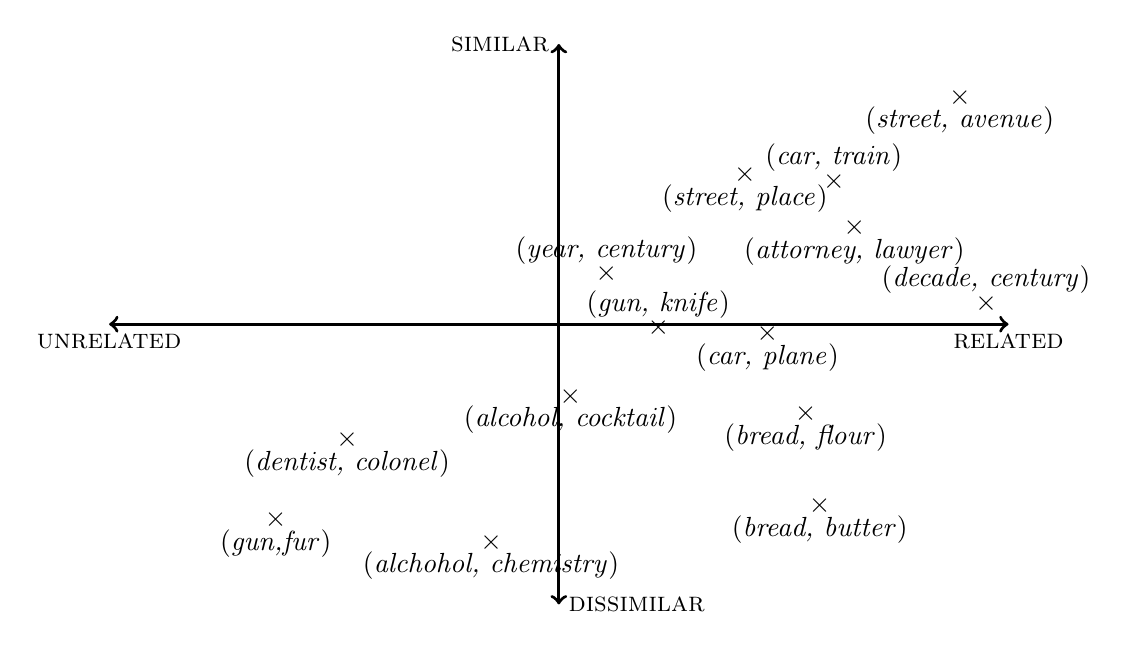
\begin{tikzpicture}
    \begin{axis}[xscale=2,yscale=1.5,hide axis]
      \addplot [<->,very thick] coordinates{(0,5) (10,5)};
      \addplot [<->,very thick] coordinates{(5,0) (5,10)};
      \node at (axis cs: 0,5) [below] {\normalsize \textsc{unrelated}};
      \node at (axis cs: 10,5) [below] {\normalsize \textsc{related}};
      \node at (axis cs: 5,0) [right] {\normalsize \textsc{dissimilar}};
      \node at (axis cs: 5,10) [left] {\normalsize \textsc{similar}};
      \node at (axis cs: 7.901,1.760) [below] {(\emph{bread, butter})};
      \node at (axis cs: 7.901,1.760) {$\times$};
      \node at (axis cs: 2.646,2.940) [below] {(\emph{dentist, colonel})};
      \node at (axis cs: 2.646,2.940) {$\times$};
      \node at (axis cs: 4.247,1.109) [below] {(\emph{alchohol, chemistry})};
      \node at (axis cs: 4.247,1.109) {$\times$};
      \node at (axis cs: 7.744,3.406) [below] {(\emph{bread, flour})};
      \node at (axis cs: 7.744,3.406) {$\times$};
      \node at (axis cs: 5.129,3.714) [below] {(\emph{alcohol, cocktail})};
      \node at (axis cs: 5.129,3.714) {$\times$};
      \node at (axis cs: 5.530,5.901) [above] {(\emph{year, century})};
      \node at (axis cs: 5.530,5.901) {$\times$};
      \node at (axis cs: 9.75,5.368) [above] {(\emph{decade, century})};
      \node at (axis cs: 9.75,5.368) {$\times$};
      \node at (axis cs: 7.320,4.828) [below] {(\emph{car, plane})};
      \node at (axis cs: 7.320,4.828) {$\times$};
      \node at (axis cs: 8.057,7.550) [above] {(\emph{car, train})};
      \node at (axis cs: 8.057,7.550) {$\times$};
      \node at (axis cs: 8.286,6.724) [below] {(\emph{attorney, lawyer})};
      \node at (axis cs: 8.286,6.724) {$\times$};
      \node at (axis cs: 1.852,1.512) [below] {(\emph{gun,fur})};
      \node at (axis cs: 1.852,1.512) {$\times$};
      \node at (axis cs: 6.106,4.936) [above] {(\emph{gun, knife})};
      \node at (axis cs: 6.106,4.936) {$\times$};
      \node at (axis cs: 7.068,7.667) [below] {(\emph{street, place})};
      \node at (axis cs: 7.068,7.667) {$\times$};
      \node at (axis cs: 9.458,9.050) [below] {(\emph{street, avenue})};
      \node at (axis cs: 9.458,9.050) {$\times$};
    \end{axis}
  \end{tikzpicture}
\caption{Noun pair scores along axes of relatedness and similarity as returned by a model built from features of 2x2 word co-occurrence window, 400 dimensional, \textsc{indy} type subspaces.}
\label{fig:axes}
\end{figure}

Putting aside for a moment the analysis of individual features, the overall import of this comparison is to a certain extent the vindication of the hypothesis that different features are predictive of relatedness versus similarity.\footnote{Intriguingly, when identical words are given as input, they are rated as being very related and very dissimilar.  The latter outcome is obviously an imperfection, but it also reveals the extent to which the models of each type of semantic phenomenon are making use of different geometric features, or the same features in opposite ways.}  This is illustrated in Figure~\ref{fig:axes}, where a selection of word pairs from both the WordSim and SimLex datasets are projected along axes of relatedness and similarity based on the outputs of the respective models learned based on the geometric features of 2x2 word window, 400 dimensional \textsc{indy} subspaces.  So, for instance, \emph{bread} is considered fairly related but not at all similar to \emph{butter}; \emph{flour} is rated as being about equally related to \emph{bread} as \emph{butter}, but somewhat more similar.  Similar trends are observed in the progress from (\emph{car, plane}) to (\emph{car, train}) and (\emph{alcohol, chemistry}) to (\emph{alcohol, cocktail}).  Meanwhile, and perhaps less explicably, \emph{year} and \emph{decade} are about equally similar to \emph{century}, but \emph{decade} is modelled as being considerably more related.  The emptiness of the upper-left region of the field in this selection is characteristic of the models overall: words that are similar are in general \emph{de facto} related to one another, but \emph{relatedness} does not conversely predict similarity.

Figure~\ref{fig:relsimspaces} presents an assortment of subspaces

\begin{figure}
\footnotesize
\begin{subfigure}{0.3\textwidth} % bread - butter
\centering
  \begin{tikzpicture}
    \def\varA{0.4845,70.1031,81.8944};
    \def\varB{62.7253,30.3505,87.3224};
    \def\varC{29.7558,29.7557,29.7557};
    \def\varM{10.9901,34.2885,43.9946};
    \def\varX{100.0506,36.9228,56.1392};
    \def\varAN{0.1348,19.5088,22.7901};
    \def\varBN{16.8439,8.1502,23.4491};
    \def\varCN{17.3205,17.3205,17.3205};
    \def\varMN{5.7994,18.0940,23.2158};
    \def\varXN{24.9048,9.1909,13.9743};
%    \def\varA{85.1680,36.1431,55.3263};
%    \def\varB{9.1985,75.2824,82.0287};
%    \def\varC{31.9558,31.9563,31.9559};
%    \def\varM{27.9114,42.4340,25.5222};
%    \def\varX{59.3150,89.9278,54.0899};
%    \def\varAN{23.7016,10.0583,15.3969};
%    \def\varBN{2.4701,20.2160,22.0276};
%    \def\varCN{17.3204,17.3206,17.3205};
%    \def\varMN{14.7309,22.3956,13.4699};
%    \def\varXN{14.7618,22.3804,13.4614};
    \begin{axis}[scale = 0.6,axis line style=white,view={120}{10},xmin=0,xmax=100,ymin=0,ymax=100,zmin=0,zmax=100,colormap/blackwhite,ticks=none]
      \addplot3[color=black,thick] coordinates {(0,0,100) (0,100,100)};
      \addplot3[color=black,thick] coordinates {(0,0,100) (100,0,100)};
      \addplot3[color=black,thick] coordinates {(0,100,0) (0,100,100)};
      \addplot3[color=black,thick] coordinates {(0,100,0) (100,100,0)};
      \addplot3[color=black,thick] coordinates {(100,0,0) (100,0,100)};
      \addplot3[color=black,thick] coordinates {(100,0,0) (100,100,0)};
      \addplot3[color=black] coordinates {(0,0,0) (0,0,100)};
      \addplot3[color=black] coordinates {(0,0,0) (0,100,0)};
      \addplot3[color=black] coordinates {(0,0,0) (100,0,0)};
      \addplot3[patch,patch type=triangle,color=gray,fill opacity=0.0] coordinates {(0.0,0.0,0.0) (\varCN) (\varAN)};
      \addplot3[patch,patch type=triangle,color=gray,fill opacity=0.0] coordinates {(0.0,0.0,0.0) (\varCN) (\varBN)};
      \addplot3[patch,patch type=triangle,color=darkgray,fill opacity=0.75] coordinates {(\varCN) (\varAN) (\varBN)};
      \addplot3[patch,patch type=triangle,color=darkgray,fill opacity=0.5] coordinates {(\varMN) (\varAN) (\varBN)};
      \addplot3[patch,patch type=triangle,color=darkgray,fill opacity=0.25] coordinates {(\varXN) (\varAN) (\varBN)};
      \addplot3 [color=black,thick] coordinates {(0,0,0) (\varCN)};
      \addplot3 [color=black,thick] coordinates {(0,0,0) (\varXN)};
      \addplot3 [color=black,thick] coordinates {(0,0,0) (\varMN)};
%      \addplot3[opacity = 0.1,surf,z buffer = sort,samples = 21,variable = \u,variable y = \v,domain = 0:90,y domain = 0:90,]
%    ({1*cos(u)*sin(v)}, {1*sin(u)*sin(v)}, {1*cos(v)});
      \addplot3 [patch,patch type=rectangle,color=lightgray,fill opacity=0.0] coordinates{(\varAN) (\varA) (\varB) (\varBN)
};
      \addplot3 [color=black,thick] coordinates {(\varCN) (\varC)};
      \addplot3 [color=black,thick] coordinates {(\varXN) (\varX)};
      \addplot3 [color=black,thick] coordinates {(\varMN) (\varM)};
      \addplot3 [patch,patch type=triangle,color=lightgray,fill opacity=0.75] coordinates{(\varA) (\varC) (\varB)};
      \addplot3 [patch,patch type=triangle,color=gray,fill opacity=0.25] coordinates{(\varA) (\varX) (\varB)};
      \addplot3 [patch,patch type=triangle,color=gray,fill opacity=0.5] coordinates{(\varA) (\varM) (\varB)};
%      \node [anchor=south] at (axis cs: 0.1,0.0,0.0) {O};
      \node [anchor=south] at (axis cs: \varA) {bread};
      \node [anchor=south] at (axis cs: \varB) {butter};
%      \node [anchor=south] at (axis cs: \varAN) {A'};
%      \node [anchor=west] at (axis cs: \varBN) {B'};
%      \node [anchor=south] at (axis cs: \varCN) {C'};
%      \draw plot [mark=*, mark size=1] coordinates{(axis cs: \varCN)};
      \node [anchor=south] at (axis cs: \varC) {C};
%      \node [anchor=east] at (axis cs: \varXN) {X'};
%      \draw plot [mark=*, mark size=1] coordinates{(axis cs: \varXN)};
      \node [anchor=south] at (axis cs: \varX) {X};
%      \node [anchor=west] at (axis cs: \varMN) {M'};
%      \draw plot [mark=*, mark size=1] coordinates{(axis cs: \varMN)};
      \node [anchor=south] at (axis cs: \varM) {M};
    \end{axis}
  \end{tikzpicture}
\caption*{\footnotesize \emph{relatedness = 7.901} \\ \emph{similarity = 1.760}}
\end{subfigure}
\hfill
\begin{subfigure}{0.3\textwidth} % car - plane
\centering
  \begin{tikzpicture}
\def\varA{-8.639,51.611,50.881};
    \def\varA{-9.246,47.099,55.012};
    \def\varB{46.777,22.683,65.128};
    \def\varC{27.435,27.435,27.434};
    \def\varM{9.784,31.783,40.743};
    \def\varX{99.192,36.477,55.514};
    \def\varAN{-3.799,19.354,22.605};
    \def\varBN{16.840,8.166,23.446};
    \def\varCN{17.321,17.321,17.320};
    \def\varMN{5.581,18.130,23.241};
    \def\varXN{24.927,9.167,13.951};
%    \def\varA{65.750,1.210,31.680};
%    \def\varB{0.965,45.932,69.528};
%    \def\varC{30.338,30.338,30.338};
%    \def\varM{29.455,29.617,31.942};
%    \def\varX{71.254,75.982,58.367};
%    \def\varAN{27.023,0.497,13.020};
%    \def\varBN{0.347,16.535,25.029};
%    \def\varCN{17.321,17.321,17.320};
%    \def\varMN{16.804,16.897,18.224};
%    \def\varXN{17.902,19.090,14.665};
%    \def\varA{68.1729,12.4169,22.9447};
%    \def\varB{0.0100,50.9479,65.9400};
%    \def\varC{29.6795,29.6798,29.6796};
%    \def\varM{27.4039,38.3811,23.2532};
%    \def\varX{62.2919,87.7658,51.7108};
%    \def\varAN{28.0184,5.1032,9.4301};
%    \def\varBN{0.0036,18.3421,23.7396};
%    \def\varCN{17.3204,17.3206,17.3205};
%    \def\varMN{15.6352,21.8981,13.2670};
%    \def\varXN{15.6508,22.0511,12.9923};
    \begin{axis}[scale = 0.6,axis line style=white,view={120}{10},xmin=0,xmax=100,ymin=0,ymax=100,zmin=0,zmax=100,colormap/blackwhite,ticks=none]
      \addplot3[color=black,thick] coordinates {(0,0,100) (0,100,100)};
      \addplot3[color=black,thick] coordinates {(0,0,100) (100,0,100)};
      \addplot3[color=black,thick] coordinates {(0,100,0) (0,100,100)};
      \addplot3[color=black,thick] coordinates {(0,100,0) (100,100,0)};
      \addplot3[color=black,thick] coordinates {(100,0,0) (100,0,100)};
      \addplot3[color=black,thick] coordinates {(100,0,0) (100,100,0)};
      \addplot3[color=black] coordinates {(0,0,0) (0,0,100)};
      \addplot3[color=black] coordinates {(0,0,0) (0,100,0)};
      \addplot3[color=black] coordinates {(0,0,0) (100,0,0)};
      \addplot3[patch,patch type=triangle,color=gray,fill opacity=0.0] coordinates {(0.0,0.0,0.0) (\varCN) (\varAN)};
      \addplot3[patch,patch type=triangle,color=gray,fill opacity=0.0] coordinates {(0.0,0.0,0.0) (\varCN) (\varBN)};
      \addplot3[patch,patch type=triangle,color=darkgray,fill opacity=0.75] coordinates {(\varCN) (\varAN) (\varBN)};
      \addplot3[patch,patch type=triangle,color=darkgray,fill opacity=0.5] coordinates {(\varMN) (\varAN) (\varBN)};
      \addplot3[patch,patch type=triangle,color=darkgray,fill opacity=0.25] coordinates {(\varXN) (\varAN) (\varBN)};
      \addplot3 [color=black,thick] coordinates {(0,0,0) (\varCN)};
      \addplot3 [color=black,thick] coordinates {(0,0,0) (\varXN)};
      \addplot3 [color=black,thick] coordinates {(0,0,0) (\varMN)};
%      \addplot3[opacity = 0.1,surf,z buffer = sort,samples = 21,variable = \u,variable y = \v,domain = 0:90,y domain = 0:90,]
%    ({1*cos(u)*sin(v)}, {1*sin(u)*sin(v)}, {1*cos(v)});
      \addplot3 [patch,patch type=rectangle,color=lightgray,fill opacity=0.0] coordinates{(\varAN) (\varA) (\varB) (\varBN)
};
      \addplot3 [color=black,thick] coordinates {(\varCN) (\varC)};
      \addplot3 [color=black,thick] coordinates {(\varXN) (\varX)};
      \addplot3 [color=black,thick] coordinates {(\varMN) (\varM)};
      \addplot3 [patch,patch type=triangle,color=lightgray,fill opacity=0.75] coordinates{(\varA) (\varC) (\varB)};
      \addplot3 [patch,patch type=triangle,color=gray,fill opacity=0.25] coordinates{(\varA) (\varX) (\varB)};
      \addplot3 [patch,patch type=triangle,color=gray,fill opacity=0.5] coordinates{(\varA) (\varM) (\varB)};
%      \node [anchor=south] at (axis cs: 0.1,0.0,0.0) {O};
      \node [anchor=south] at (axis cs: \varA) {car};
      \node [anchor=south] at (axis cs: \varB) {plane};
%      \node [anchor=south] at (axis cs: \varAN) {A'};
%      \node [anchor=west] at (axis cs: \varBN) {B'};
%      \node [anchor=south] at (axis cs: \varCN) {C'};
%      \draw plot [mark=*, mark size=1] coordinates{(axis cs: \varCN)};
      \node [anchor=south] at (axis cs: \varC) {C};
%      \node [anchor=east] at (axis cs: \varXN) {X'};
%      \draw plot [mark=*, mark size=1] coordinates{(axis cs: \varXN)};
      \node [anchor=south] at (axis cs: \varX) {X};
%      \node [anchor=west] at (axis cs: \varMN) {M'};
%      \draw plot [mark=*, mark size=1] coordinates{(axis cs: \varMN)};
      \node [anchor=south] at (axis cs: \varM) {M};
    \end{axis}
  \end{tikzpicture}
\caption*{\footnotesize \emph{relatedness = 7.320} \\ \emph{similarity = 4.828}}
\end{subfigure}
\hfill
\begin{subfigure}{0.3\textwidth} % car - train
\centering
  \begin{tikzpicture}
    \def\varA{29.3619,66.8752,24.7492};
    \def\varB{34.8883,2.9505,65.6366};
    \def\varC{28.6170,28.6166,28.6169};
    \def\varM{36.6335,24.0788,25.1374};
    \def\varX{87.7695,53.1711,58.6364};
    \def\varAN{11.4224,26.0159,9.6280};
    \def\varBN{14.0695,1.1898,26.4695};
    \def\varCN{17.3206,17.3204,17.3206};
    \def\varMN{21.7478,14.2946,14.9230};
    \def\varXN{22.2784,13.4963,14.8836};
%    \def\varA{66.2160,20.9391,33.5271};
%    \def\varB{0.0100,46.6561,57.9420};
%    \def\varC{28.4848,28.4852,28.4849};
%    \def\varM{26.9771,36.8601,21.6170};
%    \def\varX{59.8785,87.4870,52.2444};
%    \def\varAN{25.7592,8.1457,13.0427};
%    \def\varBN{0.0040,18.8151,23.3664};
%    \def\varCN{17.3204,17.3206,17.3205};
%    \def\varMN{16.0151,21.8822,12.8330};
%    \def\varXN{15.1989,22.2067,13.2611};
    \begin{axis}[scale = 0.6,axis line style=white,view={120}{10},xmin=0,xmax=100,ymin=0,ymax=100,zmin=0,zmax=100,colormap/blackwhite,ticks=none]
      \addplot3[color=black,thick] coordinates {(0,0,100) (0,100,100)};
      \addplot3[color=black,thick] coordinates {(0,0,100) (100,0,100)};
      \addplot3[color=black,thick] coordinates {(0,100,0) (0,100,100)};
      \addplot3[color=black,thick] coordinates {(0,100,0) (100,100,0)};
      \addplot3[color=black,thick] coordinates {(100,0,0) (100,0,100)};
      \addplot3[color=black,thick] coordinates {(100,0,0) (100,100,0)};
      \addplot3[color=black] coordinates {(0,0,0) (0,0,100)};
      \addplot3[color=black] coordinates {(0,0,0) (0,100,0)};
      \addplot3[color=black] coordinates {(0,0,0) (100,0,0)};
      \addplot3[patch,patch type=triangle,color=gray,fill opacity=0.0] coordinates {(0.0,0.0,0.0) (\varCN) (\varAN)};
      \addplot3[patch,patch type=triangle,color=gray,fill opacity=0.0] coordinates {(0.0,0.0,0.0) (\varCN) (\varBN)};
      \addplot3[patch,patch type=triangle,color=darkgray,fill opacity=0.75] coordinates {(\varCN) (\varAN) (\varBN)};
      \addplot3[patch,patch type=triangle,color=darkgray,fill opacity=0.5] coordinates {(\varMN) (\varAN) (\varBN)};
      \addplot3[patch,patch type=triangle,color=darkgray,fill opacity=0.25] coordinates {(\varXN) (\varAN) (\varBN)};
      \addplot3 [color=black,thick] coordinates {(0,0,0) (\varCN)};
      \addplot3 [color=black,thick] coordinates {(0,0,0) (\varXN)};
      \addplot3 [color=black,thick] coordinates {(0,0,0) (\varMN)};
%      \addplot3[opacity = 0.1,surf,z buffer = sort,samples = 21,variable = \u,variable y = \v,domain = 0:90,y domain = 0:90,]
%    ({1*cos(u)*sin(v)}, {1*sin(u)*sin(v)}, {1*cos(v)});
      \addplot3 [patch,patch type=rectangle,color=lightgray,fill opacity=0.0] coordinates{(\varAN) (\varA) (\varB) (\varBN)
};
      \addplot3 [color=black,thick] coordinates {(\varCN) (\varC)};
      \addplot3 [color=black,thick] coordinates {(\varXN) (\varX)};
      \addplot3 [color=black,thick] coordinates {(\varMN) (\varM)};
      \addplot3 [patch,patch type=triangle,color=lightgray,fill opacity=0.75] coordinates{(\varA) (\varC) (\varB)};
      \addplot3 [patch,patch type=triangle,color=gray,fill opacity=0.25] coordinates{(\varA) (\varX) (\varB)};
      \addplot3 [patch,patch type=triangle,color=gray,fill opacity=0.5] coordinates{(\varA) (\varM) (\varB)};
%      \node [anchor=south] at (axis cs: 0.1,0.0,0.0) {O};
      \node [anchor=south] at (axis cs: \varA) {car};
      \node [anchor=south] at (axis cs: \varB) {train};
%      \node [anchor=south] at (axis cs: \varAN) {A'};
%      \node [anchor=west] at (axis cs: \varBN) {B'};
%      \node [anchor=south] at (axis cs: \varCN) {C'};
%      \draw plot [mark=*, mark size=1] coordinates{(axis cs: \varCN)};
      \node [anchor=south] at (axis cs: \varC) {C};
%      \node [anchor=east] at (axis cs: \varXN) {X'};
%      \draw plot [mark=*, mark size=1] coordinates{(axis cs: \varXN)};
      \node [anchor=south] at (axis cs: \varX) {X};
%      \node [anchor=west] at (axis cs: \varMN) {M'};
%      \draw plot [mark=*, mark size=1] coordinates{(axis cs: \varMN)};
      \node [anchor=south] at (axis cs: \varM) {M};
    \end{axis}
  \end{tikzpicture}
\caption*{\footnotesize \emph{relatedness = 8.057} \\ \emph{similarity = 7.550}}
\end{subfigure}
\vfill
\vspace{10pt}
\vfill
\begin{subfigure}{0.3\textwidth} % dentist - colonel
\centering
  \begin{tikzpicture}
    \def\varA{24.4577,79.6073,0.0101};
    \def\varB{23.9986,0.0101,65.5099};
    \def\varC{29.1739,29.1740,29.1738};
    \def\varM{22.2100,33.3543,31.9578};
    \def\varX{77.1030,55.1488,63.7419};
    \def\varAN{8.8105,28.6771,0.0036};
    \def\varBN{10.3194,0.0043,28.1693};
    \def\varCN{17.3205,17.3206,17.3205};
    \def\varMN{12.9996,19.5225,18.7051};
    \def\varXN{20.2488,14.4832,16.7399};
%    \def\varA{79.5976,24.4839,0.0101};
%    \def\varB{0.0101,26.6375,64.4791};
%    \def\varC{28.6100,28.6098,28.6098};
%    \def\varM{25.9353,38.8824,21.0112};
%    \def\varX{54.9291,78.8644,61.7485};
%    \def\varAN{28.6741,8.8201,0.0036};
%    \def\varBN{0.0043,11.4546,27.7271};
%    \def\varCN{17.3206,17.3205,17.3205};
%    \def\varMN{15.1834,22.7631,12.3007};
%    \def\varXN{14.4253,20.7111,16.2162};
    \begin{axis}[scale = 0.6,axis line style=white,view={120}{10},xmin=0,xmax=100,ymin=0,ymax=100,zmin=0,zmax=100,colormap/blackwhite,ticks=none]
      \addplot3[color=black,thick] coordinates {(0,0,100) (0,100,100)};
      \addplot3[color=black,thick] coordinates {(0,0,100) (100,0,100)};
      \addplot3[color=black,thick] coordinates {(0,100,0) (0,100,100)};
      \addplot3[color=black,thick] coordinates {(0,100,0) (100,100,0)};
      \addplot3[color=black,thick] coordinates {(100,0,0) (100,0,100)};
      \addplot3[color=black,thick] coordinates {(100,0,0) (100,100,0)};
      \addplot3[color=black] coordinates {(0,0,0) (0,0,100)};
      \addplot3[color=black] coordinates {(0,0,0) (0,100,0)};
      \addplot3[color=black] coordinates {(0,0,0) (100,0,0)};
      \addplot3[patch,patch type=triangle,color=gray,fill opacity=0.0] coordinates {(0.0,0.0,0.0) (\varCN) (\varAN)};
      \addplot3[patch,patch type=triangle,color=gray,fill opacity=0.0] coordinates {(0.0,0.0,0.0) (\varCN) (\varBN)};
      \addplot3[patch,patch type=triangle,color=darkgray,fill opacity=0.75] coordinates {(\varCN) (\varAN) (\varBN)};
      \addplot3[patch,patch type=triangle,color=darkgray,fill opacity=0.5] coordinates {(\varMN) (\varAN) (\varBN)};
      \addplot3[patch,patch type=triangle,color=darkgray,fill opacity=0.25] coordinates {(\varXN) (\varAN) (\varBN)};
      \addplot3 [color=black,thick] coordinates {(0,0,0) (\varCN)};
      \addplot3 [color=black,thick] coordinates {(0,0,0) (\varXN)};
      \addplot3 [color=black,thick] coordinates {(0,0,0) (\varMN)};
%      \addplot3[opacity = 0.1,surf,z buffer = sort,samples = 21,variable = \u,variable y = \v,domain = 0:90,y domain = 0:90,]
%    ({1*cos(u)*sin(v)}, {1*sin(u)*sin(v)}, {1*cos(v)});
      \addplot3 [patch,patch type=rectangle,color=lightgray,fill opacity=0.0] coordinates{(\varAN) (\varA) (\varB) (\varBN)
};
      \addplot3 [color=black,thick] coordinates {(\varCN) (\varC)};
      \addplot3 [color=black,thick] coordinates {(\varXN) (\varX)};
      \addplot3 [color=black,thick] coordinates {(\varMN) (\varM)};
      \addplot3 [patch,patch type=triangle,color=lightgray,fill opacity=0.75] coordinates{(\varA) (\varC) (\varB)};
      \addplot3 [patch,patch type=triangle,color=gray,fill opacity=0.25] coordinates{(\varA) (\varX) (\varB)};
      \addplot3 [patch,patch type=triangle,color=gray,fill opacity=0.5] coordinates{(\varA) (\varM) (\varB)};
%      \node [anchor=south] at (axis cs: 0.1,0.0,0.0) {O};
      \node [anchor=south] at (axis cs: \varA) {dentist};
      \node [anchor=south] at (axis cs: \varB) {colonel};
%      \node [anchor=south] at (axis cs: \varAN) {A'};
%      \node [anchor=west] at (axis cs: \varBN) {B'};
%      \node [anchor=south] at (axis cs: \varCN) {C'};
%      \draw plot [mark=*, mark size=1] coordinates{(axis cs: \varCN)};
      \node [anchor=south] at (axis cs: \varC) {C};
%      \node [anchor=east] at (axis cs: \varXN) {X'};
%      \draw plot [mark=*, mark size=1] coordinates{(axis cs: \varXN)};
      \node [anchor=south] at (axis cs: \varX) {X};
%      \node [anchor=west] at (axis cs: \varMN) {M'};
%      \draw plot [mark=*, mark size=1] coordinates{(axis cs: \varMN)};
      \node [anchor=south] at (axis cs: \varM) {M};
    \end{axis}
  \end{tikzpicture}
\caption*{\footnotesize \emph{relatedness = 2.646} \\ \emph{similarity = 2.940}}
\end{subfigure}
\hfill
\begin{subfigure}{0.3\textwidth} % alcohol - cocktail
\centering
  \begin{tikzpicture}
    \def\varA{0.0441,62.0809,72.3646};
    \def\varB{48.9838,23.4812,68.0899};
    \def\varC{28.4173,28.4167,28.4161};
    \def\varM{10.4545,32.7756,42.0257};
    \def\varX{98.1159,36.1570,54.9788};
    \def\varAN{0.0139,19.5336,22.7693};
    \def\varBN{16.8709,8.0873,23.4514};
    \def\varCN{17.3209,17.3205,17.3202};
    \def\varMN{5.7748,18.1044,23.2139};
    \def\varXN{24.9155,9.1817,13.9613};
%    \def\varA{84.7123,15.1649,13.5094};
%    \def\varB{0.0100,52.2970,79.7038};
%    \def\varC{30.4733,30.4731,30.4729};
%    \def\varM{31.8383,38.7399,20.8405};
%    \def\varX{66.1332,85.0427,48.5236};
%    \def\varAN{29.1733,5.2225,4.6524};
%    \def\varBN{0.0032,16.4578,25.0827};
%    \def\varCN{17.3206,17.3205,17.3204};
%    \def\varMN{17.5894,21.4022,11.5135};
%    \def\varXN{16.7916,21.5928,12.3204};
    \begin{axis}[scale = 0.6,axis line style=white,view={120}{10},xmin=0,xmax=100,ymin=0,ymax=100,zmin=0,zmax=100,colormap/blackwhite,ticks=none]
      \addplot3[color=black,thick] coordinates {(0,0,100) (0,100,100)};
      \addplot3[color=black,thick] coordinates {(0,0,100) (100,0,100)};
      \addplot3[color=black,thick] coordinates {(0,100,0) (0,100,100)};
      \addplot3[color=black,thick] coordinates {(0,100,0) (100,100,0)};
      \addplot3[color=black,thick] coordinates {(100,0,0) (100,0,100)};
      \addplot3[color=black,thick] coordinates {(100,0,0) (100,100,0)};
      \addplot3[color=black] coordinates {(0,0,0) (0,0,100)};
      \addplot3[color=black] coordinates {(0,0,0) (0,100,0)};
      \addplot3[color=black] coordinates {(0,0,0) (100,0,0)};
      \addplot3[patch,patch type=triangle,color=gray,fill opacity=0.0] coordinates {(0.0,0.0,0.0) (\varCN) (\varAN)};
      \addplot3[patch,patch type=triangle,color=gray,fill opacity=0.0] coordinates {(0.0,0.0,0.0) (\varCN) (\varBN)};
      \addplot3[patch,patch type=triangle,color=darkgray,fill opacity=0.75] coordinates {(\varCN) (\varAN) (\varBN)};
      \addplot3[patch,patch type=triangle,color=darkgray,fill opacity=0.5] coordinates {(\varMN) (\varAN) (\varBN)};
      \addplot3[patch,patch type=triangle,color=darkgray,fill opacity=0.25] coordinates {(\varXN) (\varAN) (\varBN)};
      \addplot3 [color=black,thick] coordinates {(0,0,0) (\varCN)};
      \addplot3 [color=black,thick] coordinates {(0,0,0) (\varXN)};
      \addplot3 [color=black,thick] coordinates {(0,0,0) (\varMN)};
%      \addplot3[opacity = 0.1,surf,z buffer = sort,samples = 21,variable = \u,variable y = \v,domain = 0:90,y domain = 0:90,]
%    ({1*cos(u)*sin(v)}, {1*sin(u)*sin(v)}, {1*cos(v)});
      \addplot3 [patch,patch type=rectangle,color=lightgray,fill opacity=0.0] coordinates{(\varAN) (\varA) (\varB) (\varBN)
};
      \addplot3 [color=black,thick] coordinates {(\varCN) (\varC)};
      \addplot3 [color=black,thick] coordinates {(\varXN) (\varX)};
      \addplot3 [color=black,thick] coordinates {(\varMN) (\varM)};
      \addplot3 [patch,patch type=triangle,color=lightgray,fill opacity=0.75] coordinates{(\varA) (\varC) (\varB)};
      \addplot3 [patch,patch type=triangle,color=gray,fill opacity=0.25] coordinates{(\varA) (\varX) (\varB)};
      \addplot3 [patch,patch type=triangle,color=gray,fill opacity=0.5] coordinates{(\varA) (\varM) (\varB)};
%      \node [anchor=south] at (axis cs: 0.1,0.0,0.0) {O};
      \node [anchor=south] at (axis cs: \varA) {cocktail};
      \node [anchor=south] at (axis cs: \varB) {alcohol};
%      \node [anchor=south] at (axis cs: \varAN) {A'};
%      \node [anchor=west] at (axis cs: \varBN) {B'};
%      \node [anchor=south] at (axis cs: \varCN) {C'};
%      \draw plot [mark=*, mark size=1] coordinates{(axis cs: \varCN)};
      \node [anchor=south] at (axis cs: \varC) {C};
%      \node [anchor=east] at (axis cs: \varXN) {X'};
%      \draw plot [mark=*, mark size=1] coordinates{(axis cs: \varXN)};
      \node [anchor=south] at (axis cs: \varX) {X};
%      \node [anchor=west] at (axis cs: \varMN) {M'};
%      \draw plot [mark=*, mark size=1] coordinates{(axis cs: \varMN)};
      \node [anchor=south] at (axis cs: \varM) {M};
    \end{axis}
  \end{tikzpicture}
\caption*{\footnotesize \emph{relatedness = 5.129} \\ \emph{similarity = 3.714}}
\end{subfigure}
\hfill
\begin{subfigure}{0.3\textwidth} % bread - flour
\centering
  \begin{tikzpicture}
    \def\varA{0.5080,73.6638,86.0712};
    \def\varB{61.6190,29.8353,85.7887};
    \def\varC{29.6193,29.6192,29.6193};
    \def\varM{10.9373,34.1320,43.7940};
    \def\varX{99.2437,36.6311,55.6956};
    \def\varAN{0.1345,19.5065,22.7921};
    \def\varBN{16.8423,8.1549,23.4486};
    \def\varCN{17.3205,17.3205,17.3205};
    \def\varMN{5.7981,18.0941,23.2161};
    \def\varXN{24.9035,9.1919,13.9759};
%    \def\varA{85.556,38.144,57.211};
%    \def\varB{11.017,76.327,82.984};
%    \def\varC{31.802,31.802,31.802};
%    \def\varM{27.658,42.287,25.461};
%    \def\varX{58.701,89.297,53.661};
%    \def\varAN{23.384,10.425,15.637};
%    \def\varBN{2.918,20.213,21.976};
%    \def\varCN{17.320,17.321,17.320};
%    \def\varMN{14.665,22.421,13.500};
%    \def\varXN{14.727,22.403,13.462};
    \begin{axis}[scale = 0.6,axis line style=white,view={120}{10},xmin=0,xmax=100,ymin=0,ymax=100,zmin=0,zmax=100,colormap/blackwhite,ticks=none]
      \addplot3[color=black,thick] coordinates {(0,0,100) (0,100,100)};
      \addplot3[color=black,thick] coordinates {(0,0,100) (100,0,100)};
      \addplot3[color=black,thick] coordinates {(0,100,0) (0,100,100)};
      \addplot3[color=black,thick] coordinates {(0,100,0) (100,100,0)};
      \addplot3[color=black,thick] coordinates {(100,0,0) (100,0,100)};
      \addplot3[color=black,thick] coordinates {(100,0,0) (100,100,0)};
      \addplot3[color=black] coordinates {(0,0,0) (0,0,100)};
      \addplot3[color=black] coordinates {(0,0,0) (0,100,0)};
      \addplot3[color=black] coordinates {(0,0,0) (100,0,0)};
      \addplot3[patch,patch type=triangle,color=gray,fill opacity=0.0] coordinates {(0.0,0.0,0.0) (\varCN) (\varAN)};
      \addplot3[patch,patch type=triangle,color=gray,fill opacity=0.0] coordinates {(0.0,0.0,0.0) (\varCN) (\varBN)};
      \addplot3[patch,patch type=triangle,color=darkgray,fill opacity=0.75] coordinates {(\varCN) (\varAN) (\varBN)};
      \addplot3[patch,patch type=triangle,color=darkgray,fill opacity=0.5] coordinates {(\varMN) (\varAN) (\varBN)};
      \addplot3[patch,patch type=triangle,color=darkgray,fill opacity=0.25] coordinates {(\varXN) (\varAN) (\varBN)};
      \addplot3 [color=black,thick] coordinates {(0,0,0) (\varCN)};
      \addplot3 [color=black,thick] coordinates {(0,0,0) (\varXN)};
      \addplot3 [color=black,thick] coordinates {(0,0,0) (\varMN)};
%      \addplot3[opacity = 0.1,surf,z buffer = sort,samples = 21,variable = \u,variable y = \v,domain = 0:90,y domain = 0:90,]
%    ({1*cos(u)*sin(v)}, {1*sin(u)*sin(v)}, {1*cos(v)});
      \addplot3 [patch,patch type=rectangle,color=lightgray,fill opacity=0.0] coordinates{(\varAN) (\varA) (\varB) (\varBN)
};
      \addplot3 [color=black,thick] coordinates {(\varCN) (\varC)};
      \addplot3 [color=black,thick] coordinates {(\varXN) (\varX)};
      \addplot3 [color=black,thick] coordinates {(\varMN) (\varM)};
      \addplot3 [patch,patch type=triangle,color=lightgray,fill opacity=0.75] coordinates{(\varA) (\varC) (\varB)};
      \addplot3 [patch,patch type=triangle,color=gray,fill opacity=0.25] coordinates{(\varA) (\varX) (\varB)};
      \addplot3 [patch,patch type=triangle,color=gray,fill opacity=0.5] coordinates{(\varA) (\varM) (\varB)};
%      \node [anchor=south] at (axis cs: 0.1,0.0,0.0) {O};
      \node [anchor=south] at (axis cs: \varA) {flour};
      \node [anchor=south] at (axis cs: \varB) {bread};
%      \node [anchor=south] at (axis cs: \varAN) {A'};
%      \node [anchor=west] at (axis cs: \varBN) {B'};
%      \node [anchor=south] at (axis cs: \varCN) {C'};
%      \draw plot [mark=*, mark size=1] coordinates{(axis cs: \varCN)};
      \node [anchor=south] at (axis cs: \varC) {C};
%      \node [anchor=east] at (axis cs: \varXN) {X'};
%      \draw plot [mark=*, mark size=1] coordinates{(axis cs: \varXN)};
      \node [anchor=south] at (axis cs: \varX) {X};
%      \node [anchor=west] at (axis cs: \varMN) {M'};
%      \draw plot [mark=*, mark size=1] coordinates{(axis cs: \varMN)};
      \node [anchor=south] at (axis cs: \varM) {M};
    \end{axis}
  \end{tikzpicture}
\caption*{\footnotesize \emph{relatedness = 7.744} \\ \emph{similarity = 3.406}}
\end{subfigure}
\caption{Subspaces, including word-vectors and generic features, derived from word pairs with an assortment of relatedness and similarity scores.}
\label{fig:relsimspaces}
\end{figure}

The contrasting 

Moving up the scale of similarity from (\emph{butter, bread}) to (\emph{plane, car}), we can observe a tightening of the angle between the word-vectors and a general contractin of the space, followed by an increase in the span between the word-vectors as we ratchet our way up to the highly similar (\emph{train, car}).  An almost opposite effect can be observed, on the other hand, as relatedness increases from (\emph{alcohol, cocktail}) to (\emph{bread, flour}), with the word-vectors themselves looming as the angle at $C$ contracts and the ratios of the distances to $M$ even out.  Perhaps the most interesting effect of all, though, is the visually evident similarity in the geometries of (\emph{colonel, dentist}), which are equivalently dissimilar and unrelated, and (\emph{train, car}), which are conversely highly similar and highly related: while my projection technique clearly struggles to accommodate the expanse of the angle between the unrelated word-vectors, the congruity of the characteristic spread of the various points in the spaces selected by the word-vectors is striking.  This raises an intriguing possibility that there may be a certain consistency in geometry based on the balance of similarity and relatedness, or, to put it differently, an indication that there is a certain shape to the statistics of a space in which similarity is the primary axis of relatedness, regardless of degree, versus a space in which there is some other specific semantic relationship in play.

\section{Frames of Similarity} \label{sec:frames}
\cite{Tversky1977}, in his psychologically motivated reflections on the geometry of similarity, observes that relationships of similarity are fundamentally not symmetric: there tends to be a preference to consider the specific more similar to the general, and the peripheral more similar to the prototypical, than the other way around.  So, to use Tversky's own example, \emph{ellipse} is more similar to \emph{circle} than \emph{circle} is to \emph{ellipse}; we might extend this conjecture to predict that \emph{wolf} is more similar to \emph{dog}, \emph{radiologist} more similar to \emph{doctor}, and \emph{limping} more similar to \emph{walking} than the converse propositions.  Indeed, the frequentist axiom extrapolated through the geometric analysis of the previous section, stating that more common words denote things that are more likely to generally be a component of a similarity relationship, is broadly in line with this observation.  Tversky makes the point that the conventional conditions of geometric relationships -- \emph{minimality}, \emph{symmetry}, and \emph{the triangle inequality} -- do not pertain in the case of similarity judgements, a point which if taken seriously serves to foil the project of a vector space model of word similarity.

\cite{ChenEA2017} carry this point forward experimentally, demonstrating that potential for the arbitrary construction of, for instance, analogies which demand geometrically impossible triangulations: to use one of their examples, \emph{nurse:patient::mother:baby} is a reasonable set of relationships, as is \emph{mother:baby::frog:tadpole}, but the proposition \emph{nurse:patient::frog:tadpole} seems obscure at best.  \citeauthor{ChenEA2017} demonstrate that human raters generally identify the failure of the third set of pairings in these types of triads, whereas standard distributional semantics including \texttt{word2vec} don't---in fact, they can't, since the semantic relationships in these models are represented as static quantities.  The point that emerges here is that semantic relationship emerge within a certain frame of reference, and the reason that the analogy comparing nurses to frogs fails is because both the axis of \textsc{caring} that sustains the connection between nurses and mothers and the axis of \textsc{parentage} that connects mothers and frogs have dropped away.

The role of frames in theories of lexical semantics has already been mentioned in Chapter~\ref{sec:lexsem}.  To reiterate the point raised there, \cite{BarsalouEA1993} proposes that cognition is organised in terms of frames allowing for a \emph{situated}, \emph{local} representations of concepts: a concept gains its structure through a situationally specific indexing of a variety of established models.  One of the consequences of this framework is that a concept emerges as the ``collection of all all specialized models for a particular type of individual, together with their associated generic situations,'' (p. XXX

So, for instance, the concept \textsc{profession} contains models for constituents such as \textsc{dentist} and \textsc{attorney} and so forth, and the conceptual scheme is structured in such a way as to offer information about the situations which both independently and jointly pertain to the models associated with those constituents.

These types of conceptual contexts are evident in the relatedness and similarity datasets which have been explored in this chapter.  In the SimLex data, for instance, (\emph{dentist}, \emph{colonel}) is rated as one of the least similar word pairs at 0.40, while (\emph{attorney}, \emph{lawyer}) is, at 9.25, considered one of the most similar pairs.  The difference seems reasonable enough in terms of a comparison between the two pairs, but the low rating of (\emph{dentist}, \emph{colonel}) leaves little room for either dentists or colonels to be even less similar to, say, gorillas, or electricity, or democracy, and so forth.  What seems to be happening here is that human evaluators are identifying an implicit conceptual frame in which each word pair is to be evaluated: in the case of attorneys, lawyers, dentists, and colonels, the frame is something like \textsc{profession}, and so the professional activities of colonels and dentists are judged to be more or less orthogonal, while attorneys and lawyers pursue very similar careers.  The inclusion of some additional comparison, for instance (\emph{dentist}, \emph{grandparent}), would suggest a broadening of the conceptual frame to something like \textsc{human}, and a corresponding drawing together of words denoting professions in particular.

Moreover, it is not particularly clear how a pair such as (\emph{dentist}, \emph{colonel}) should be considered either more or less similar to a pair like (\emph{gun}, \emph{fur}); the comparisons being made here seem just categorically different, and so the project of ranking the similarity of one above the other becomes a bit obscure.\footnote{It's tempting to apply the idiom \emph{comparing apples to oranges} here, but this phrase itself actually serves to further illustrate the point, as I would hope that my model would return a fairly high similarity score for these two fruits.}  Instead, the task at hand really seems to be to determine the conceptual domain in which the comparison is being made, and then to make an inherently relativistic judgement about the proximity of the denotations within the semantic space of that domain.  I suggest that my models are beginning to do this.  By taking a subset of co-occurrence dimensions expected to exhibit a degree of saliency for either or both of the words being analysed, a subspace with a certain degree of conceptual interpretability is generated.  So collectively, the co-occurrence terms that are jointly most predictive of 

EXAMPLES

What begins to emerge is something like a very rough version of the conceptual spaces described by \cite{Gardenfors2000}, in which regions of a space correspond to conceptual constituents and directions within regions can be interpreted as corresponding to values of properties that determine membership.  It must be emphasised that this comparison is at a general level of abstraction: my subspaces do not at this stage contain any of the nuanced attributional information of G\"{a}rdenfors's conceptual spaces, and my methodology generates unique subspaces for each word pair, so the scores returned by the models learned through linear regression are effectively comparisons between different, albeit potentially overlapping, subspaces.  Nonetheless, the reliably distinct respective predictors of relatedness and similarity within any given subspace suggest that there is already an element of conceptual structure at play in my models, even if it lacks much depth in terms of dimensional interpretation.

\cite{FaruquiEA2016} raise a number of issues with relatedness and similarity datasets, among them the uncertainty surrounding specific semantic phenomena and the lack of applicability of quantified word pair scores to practical NLP tasks.  Those authors ultimately propose that quantitative evaluations of vector space models of word meaning should avoid claims of generality, instead treating particular models as task specific implementations.  There is something to be said for this approach, and even more to be said in support of the effort to apply statistical NLP techniques to activities in other fields where heterogeneous data and contextual complexity present potentially confounding factors to the relatively abstract and rigid representational structures of distributional semantic models.  All the same, I maintain that word association tasks, particular a battery of tasks spanning a variety of semantic phenomena, can be a productive tool for exploring the capabilities of a methodology, and present the work that has been described in this chapter as a case in point.

A productive next step would be to develop methods targeting the classification of conceptual domains within which word pair comparisons are being performed, so, for instance, to identify that (\emph{dentist}, \emph{colonel}) and (\emph{attorney}, \emph{lawyer}) are both implicitly comparisons between \textsc{professions}, or at least are comparisons within the same unspecified domain.  Existing work in the field on conceptual entailment may prove helpful here: \cite{HerbelotEA2013}, for instance, use an entropic analysis of co-occurrence statistics to conjecture about hypernymy relationships between sets of words, while \cite{MelamudEA2014} use a method utilising syntagmatic co-occurrence information to model the probability of words belonging to the same semantic domain.  Equipped with an effective method for clustering relationships between words into conceptual domains, or alternatively for rating the degree of relevance inherent in a comparison between two relatedness judgements, my methodology offers, as has been demonstrated in the experiments reported above, a capacity for contextualising the relationships between representation in terms of co-occurrence dimensions and then discovering various geometric axes corresponding to different semantic properties.  As the words used as input to define a subspace become more related, the space itself likewise becomes more conceptually coherent, and I predict that these broadly semantic axes will take on a more narrowly G\"{a}rdenforsian characteristic, allowing for interpretation as properties specific to the concept implicit in the grouping.

The \textsc{indy} dimensional selection technique in particular would lend itself to this type of programmatic extension of research into semantic relatedness, as it facilitates the open-ended concatenation of dimensions from an analysis of an arbitrarily large set of constituent word-vectors (the \textsc{joint} and \textsc{indy} techniques, on the other hand, would presumably return increasingly uninteresting dimensions with universally non-zero values as the set of input words expands).  A subspace built using the \textsc{indy} technique based on an analysis of a set of words denoting, for instance, constituents of the concept \textsc{professionals} would acquire co-occurrence dimensions specifically salient to each of the input terms, and the construal of other word-vectors in the space along the collective profile of dimensions would, I forecast, be indicative of their conceptual situation according to the various properties of being a professional.  In such a space, we might predict that we would find, for instance, \emph{surgeon} somewhere in the vicinity of the region between \emph{barber} and \emph{butcher}

This proposition entails a major research project.  The data for establishing groups of conceptual relationships needs to be established, and the evaluation of a model's ability to capture the attributes giving these relationships structure presents a daunting task due to the open-endedness of conceptualisation itself.  Ultimately, questions of the validity of the assignment of properties to concepts, as they begin to reflect the modelling of situations in the world, are probably better suited for a qualitative analysis, and it is easy to imagine how this work might eventually lend itself to fruitful collaboration with fields such as education and the digital humanities.  For now I will leave this line of enquiry where it stands, with some promising results regarding the ability of my methodology to model the overlapping semantic phenomena of relatedness and similarity in a single space.  In the next chapter, I will explore my models capacity for handling a broad and important set of semantic phenomena for which I believe it will be particularly well suited: figurative language.

(for comparison, see where the pair (\emph{dentist, colonel}) falls in the space of Figure~\ref{fig:axes}, where it is one of the very few pairs considered to be marginally more similar than related)
